\documentclass{beamer}
\usepackage{graphicx, animate, caption}
\graphicspath{ {images/} }
\usetheme{Marburg}
\title{Why Meteors Rock}
\subtitle{An analysis of radio meteor detection}
\author{Charles Powell}
\institute{Exeter Mathematics School}
\date{30$^{th}$ March, 2017}

%\newcommand{\credit}[1]{\par\hfill \footnotesize Credit:~\itshape#1}
\newcommand{\credit}[1]{\hspace*{15pt}\hbox{\scriptsize Credit:\thinspace{\small\itshape #1}}}

\begin{document}
	\section{Introduction}
	\begin{frame}
		\titlepage
	\end{frame}

	\section{What is a meteor?}
	\begin{frame}
		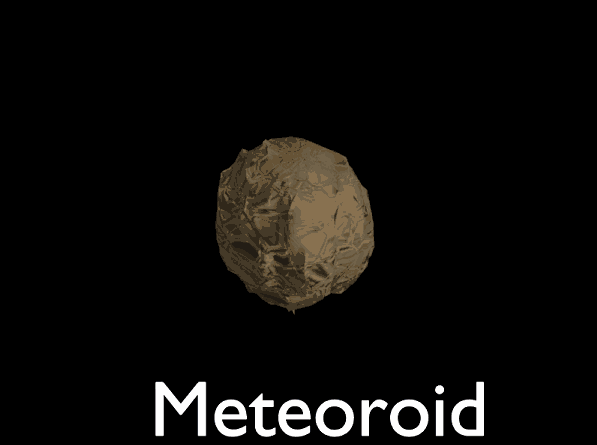
\includegraphics[width=\linewidth]{meteoroid}\\
		\credit{Wikipedia}
	\end{frame}

	\begin{frame}
		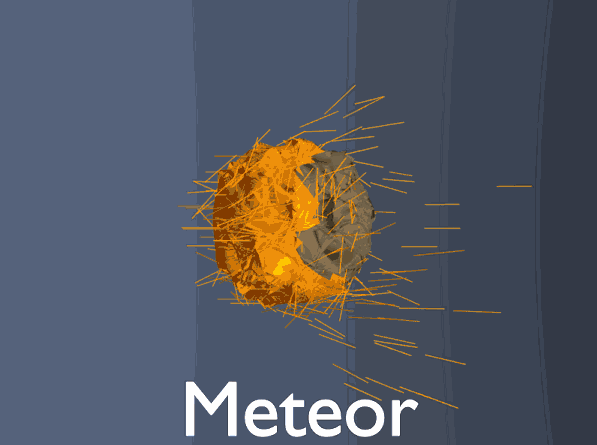
\includegraphics[width=\linewidth]{meteor}\\
		\credit{Wikipedia}
	\end{frame}	

	\begin{frame}
		
\includegraphics[width=\linewidth]{meteorite}\\
		\credit{Wikipedia}
	\end{frame}

	\section{Meteor showers}
	\begin{frame}
		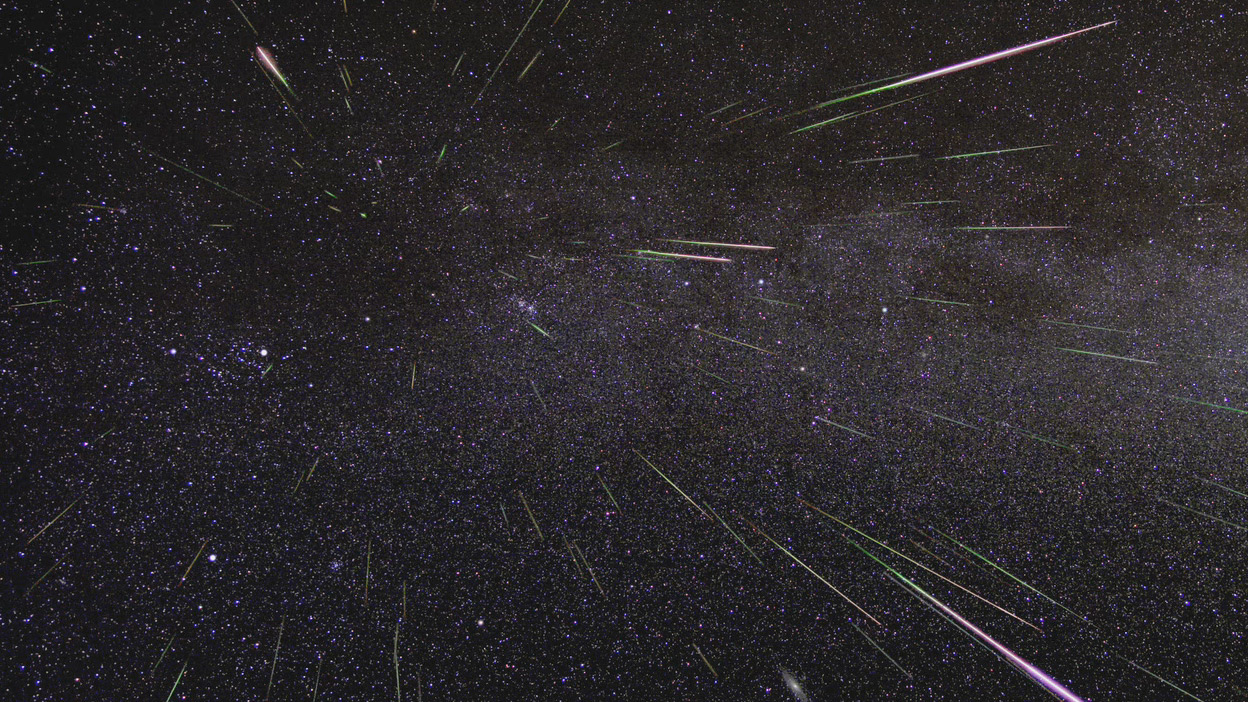
\includegraphics[width=\linewidth]{shower}\\
		\credit{nasa.gov}
	\end{frame}

	\begin{frame}
		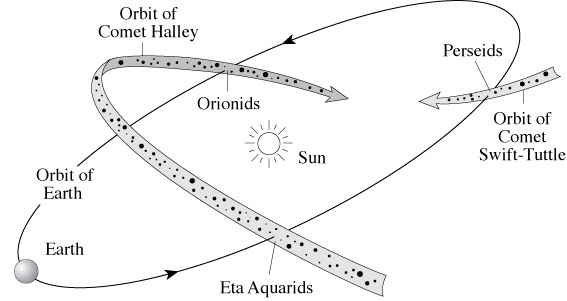
\includegraphics[width=\linewidth]{stream}\\
		\credit{NASA's Cosmos (\url{ase.tufts.edu})}
	\end{frame}

	\begin{frame}
		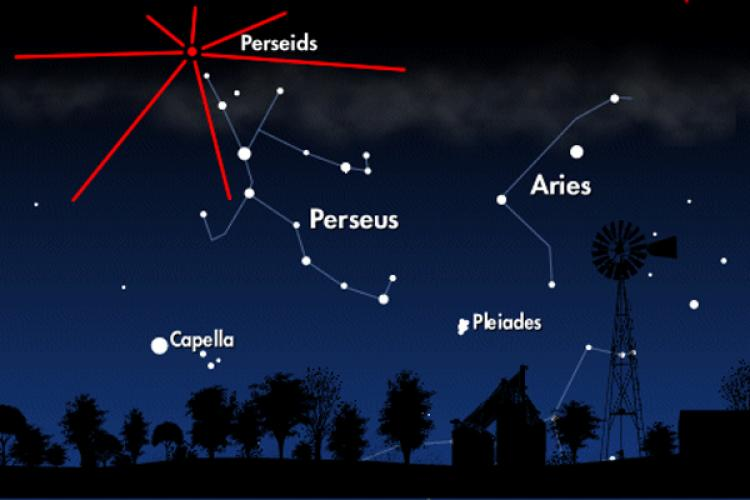
\includegraphics[width=\linewidth]{perseids}\\
		\credit{NASA}
	\end{frame}

	\begin{frame}
		\centering
		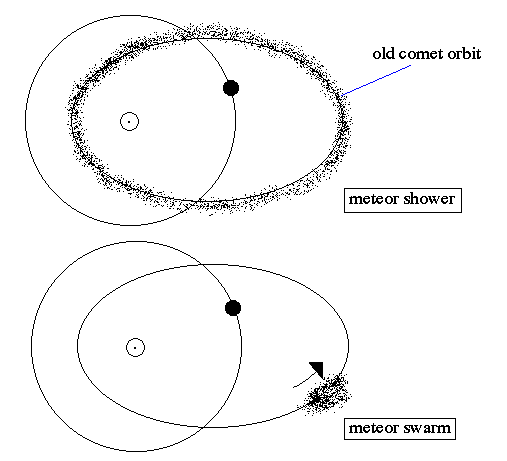
\includegraphics[width=0.8\linewidth]{stream_spread}\\
		\flushleft\credit{Oregon University}
	\end{frame}

	\section{Radio meteor detection}
	\begin{frame}
		\centering
		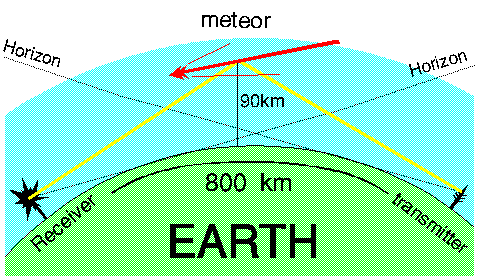
\includegraphics[width=0.7\linewidth]{detection}\\
		\flushleft\credit{Sky Scan}
	\end{frame}

	\begin{frame}
		\centering
		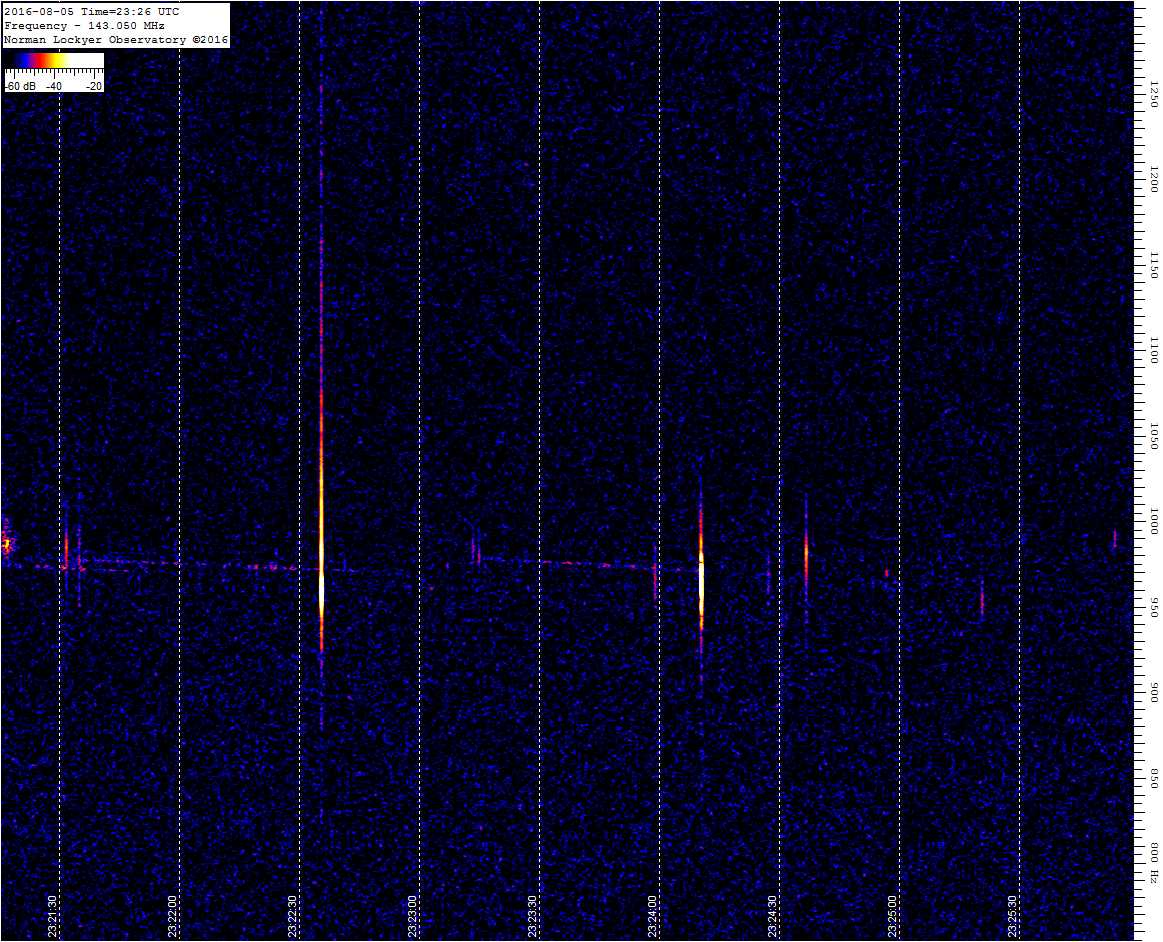
\includegraphics[width=0.55\linewidth]{2D}
		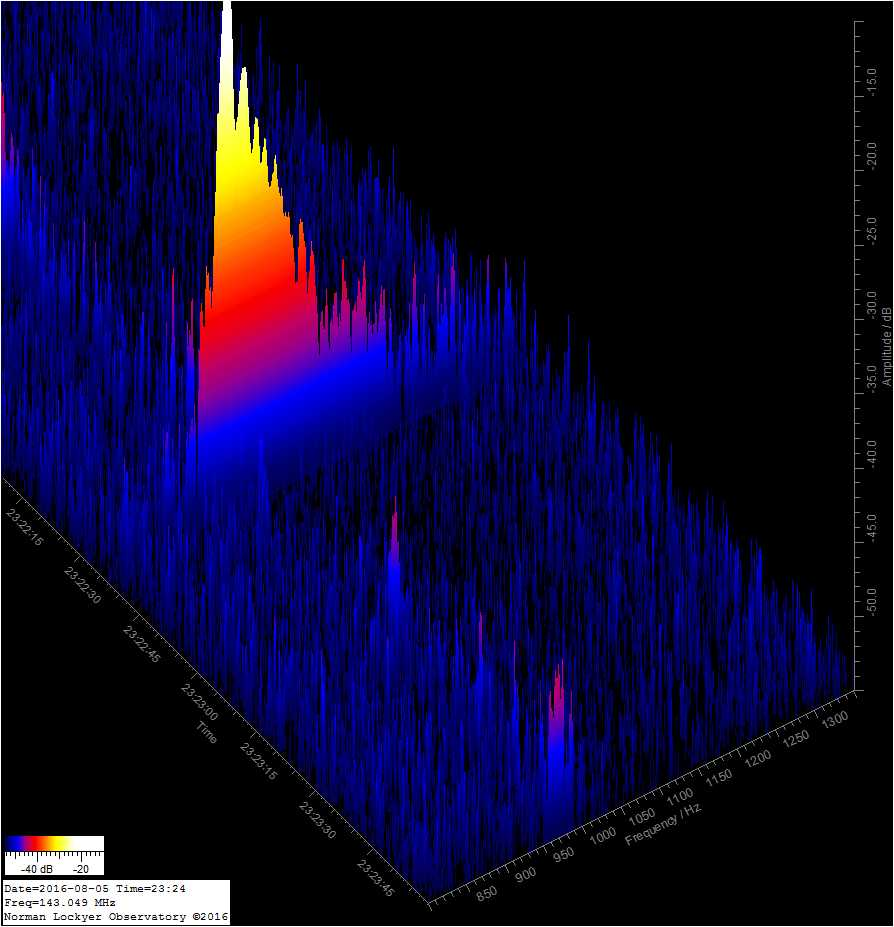
\includegraphics[width=0.43\linewidth]{3D}\\
		\flushleft\credit{Lockyer Technology Centre, NLO}
	\end{frame}

	\section{Antenna variation}
	\begin{frame}
		\centering
		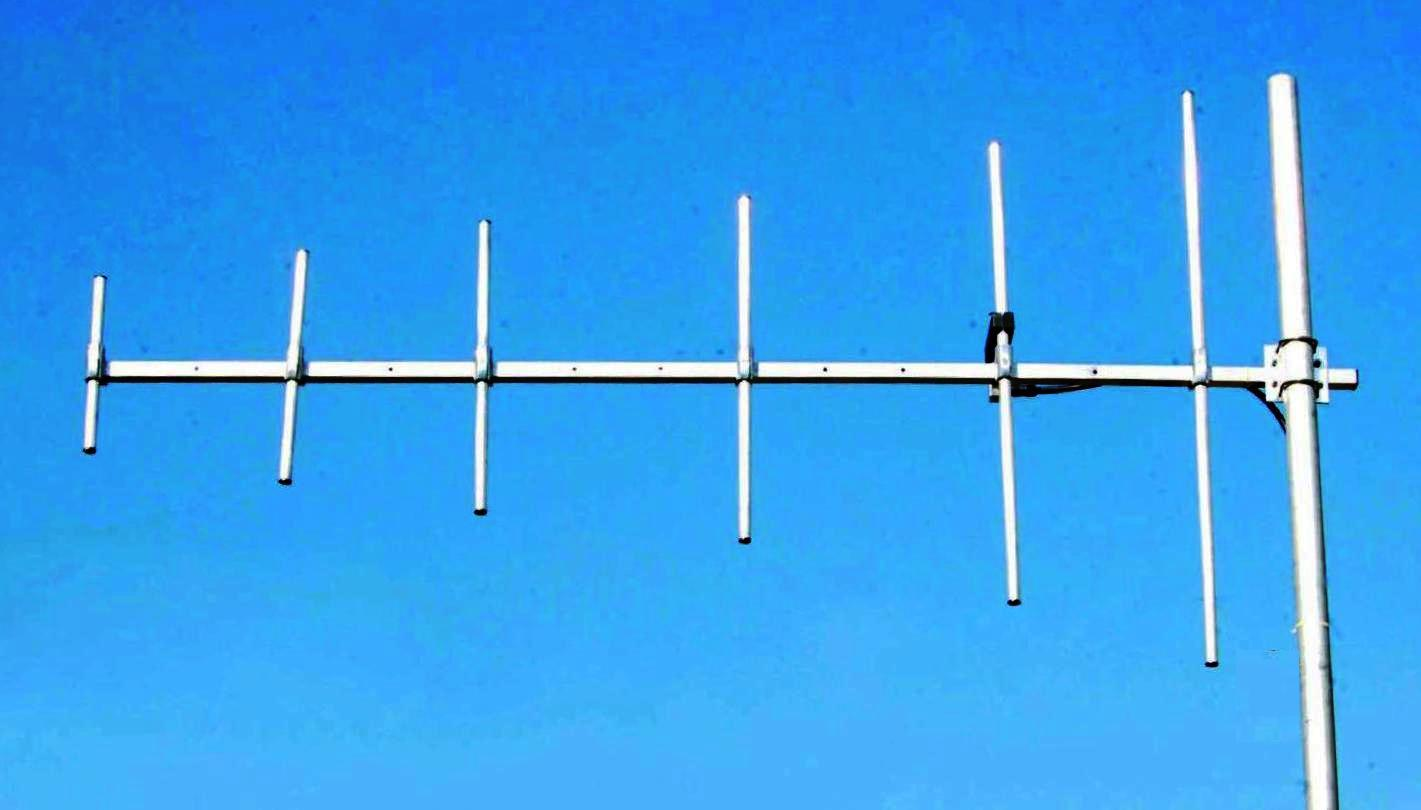
\includegraphics[width=\linewidth]{yagi}
		\credit{RF \& Antenna Resource}
	\end{frame}

	\begin{frame}
		\centering
		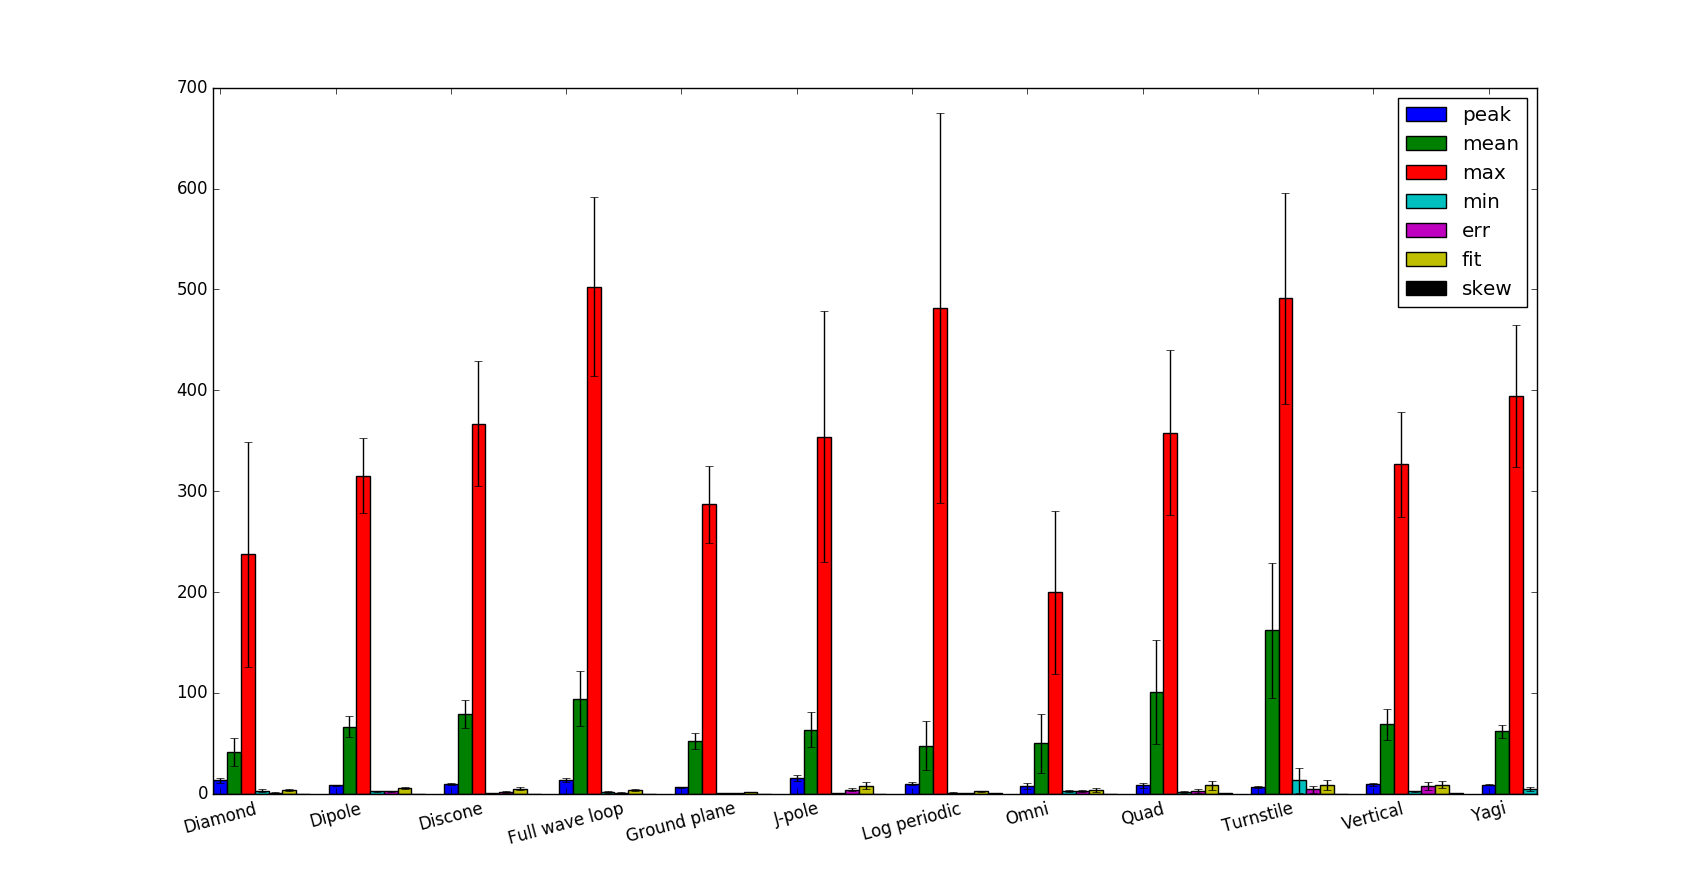
\includegraphics[width=0.85\linewidth]{antenna_large.png}\\
		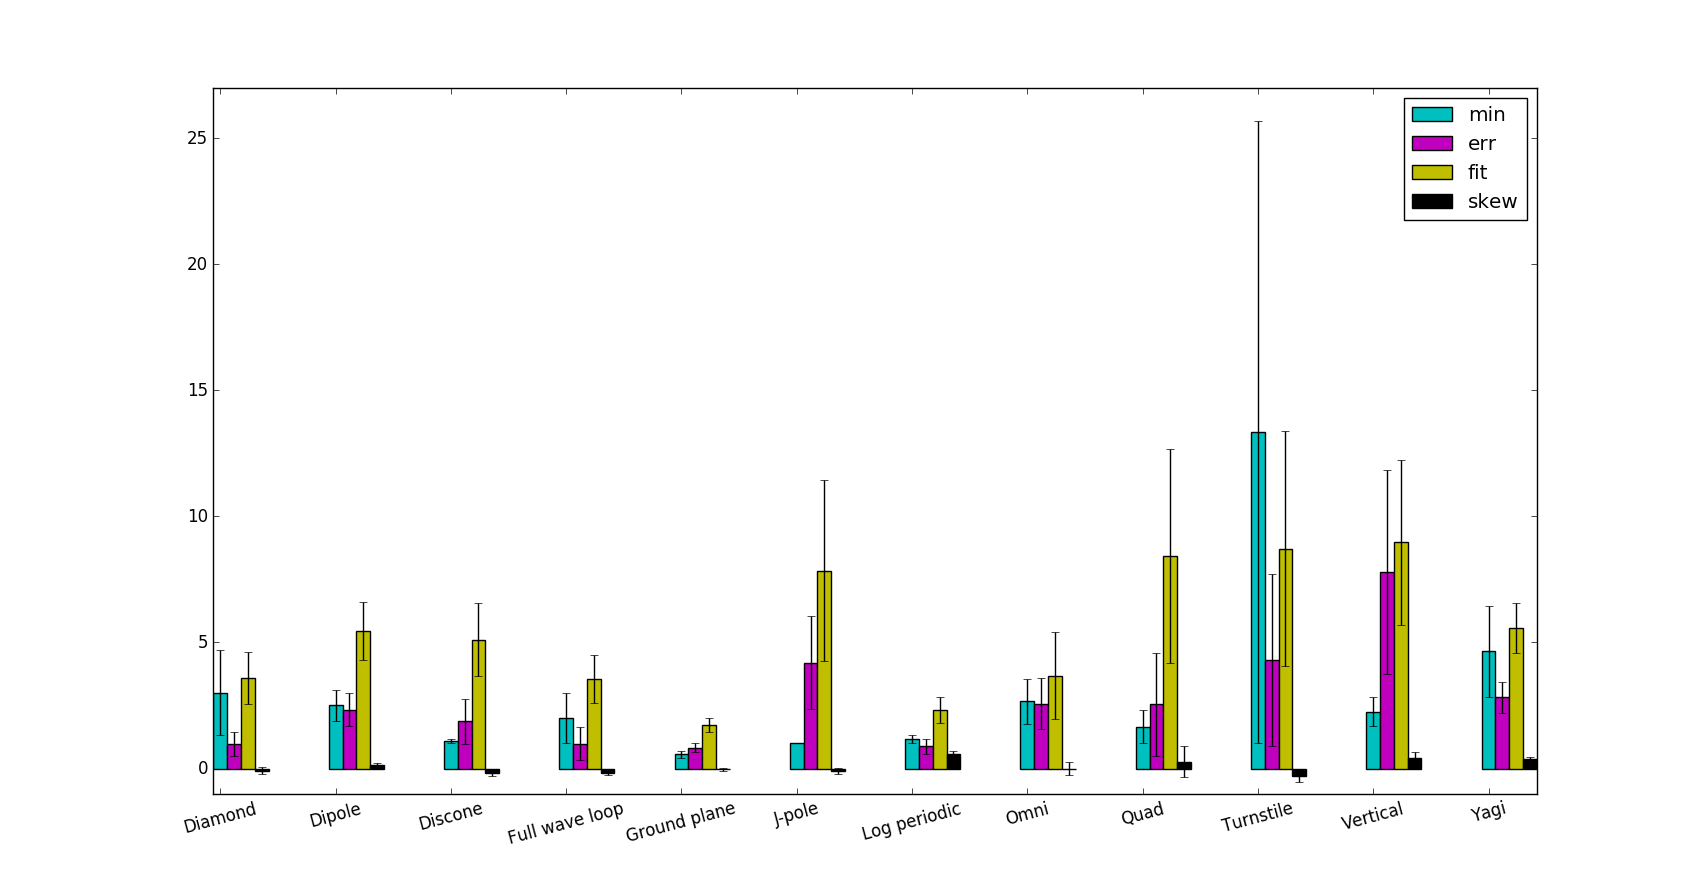
\includegraphics[width=0.85\linewidth]{antenna_small.png}
	\end{frame}
	
	\section{Spatial variation}
	\begin{frame}
		\centering
		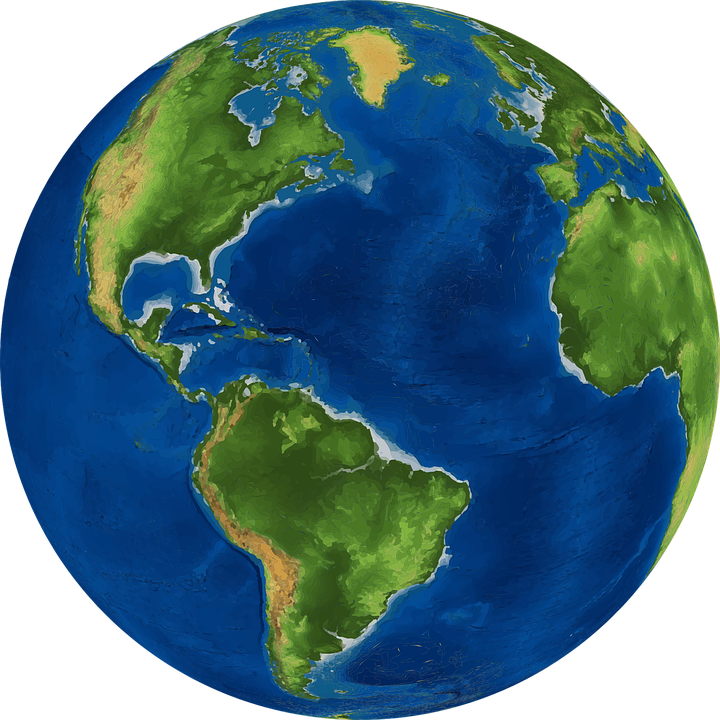
\includegraphics[width=0.6\linewidth]{spatial}\\
		\flushleft\credit{Pixabay}
	\end{frame}

	\begin{frame}
		\centering
		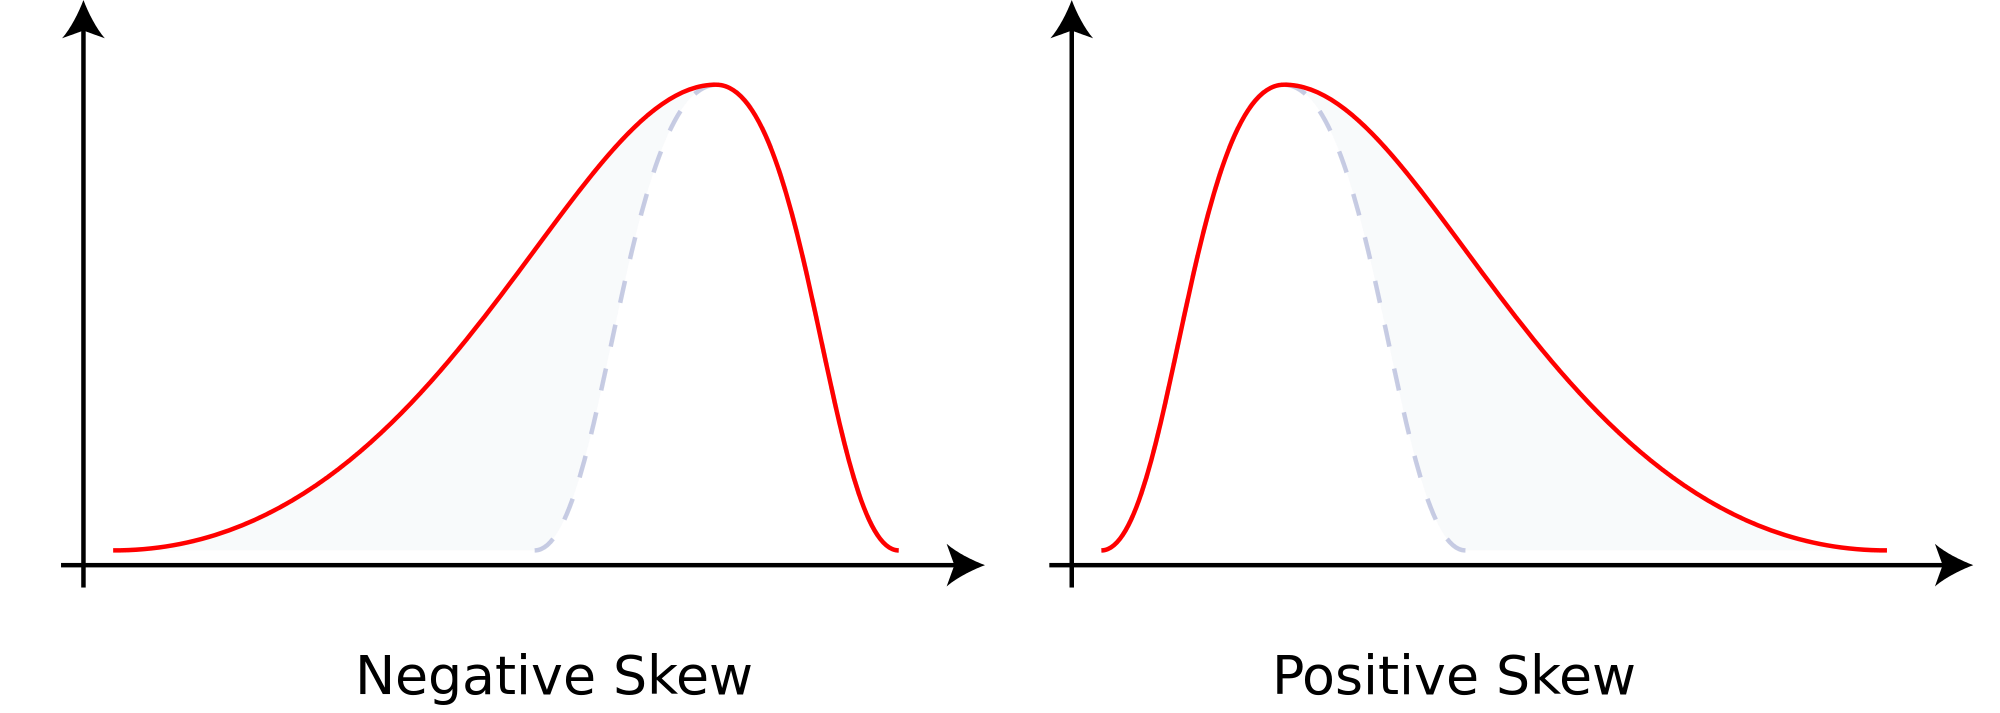
\includegraphics[width=\linewidth]{skew}\\
		\flushleft\credit{Wikipedia}
	\end{frame}
	
	\begin{frame}
		\centering
		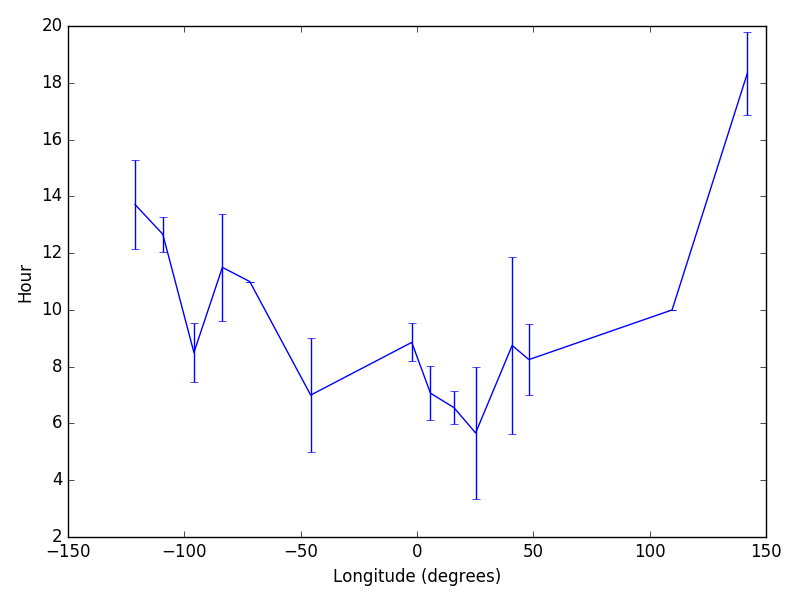
\includegraphics[width=\linewidth]{peak}
	\end{frame}
	
	\section{Diurnal shift}
	\begin{frame}
		\centering
		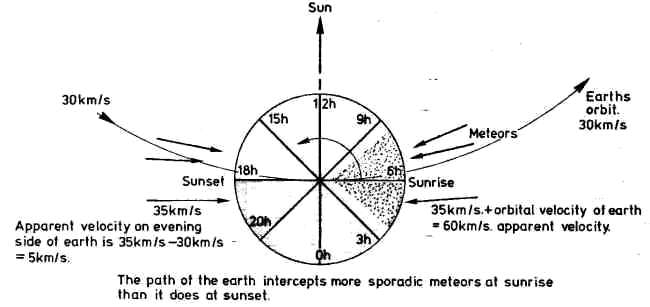
\includegraphics[width=0.8\linewidth]{img59}\\
		\flushleft\credit{British Astronomical Association}
	\end{frame}
	
	\begin{frame}
		\centering
		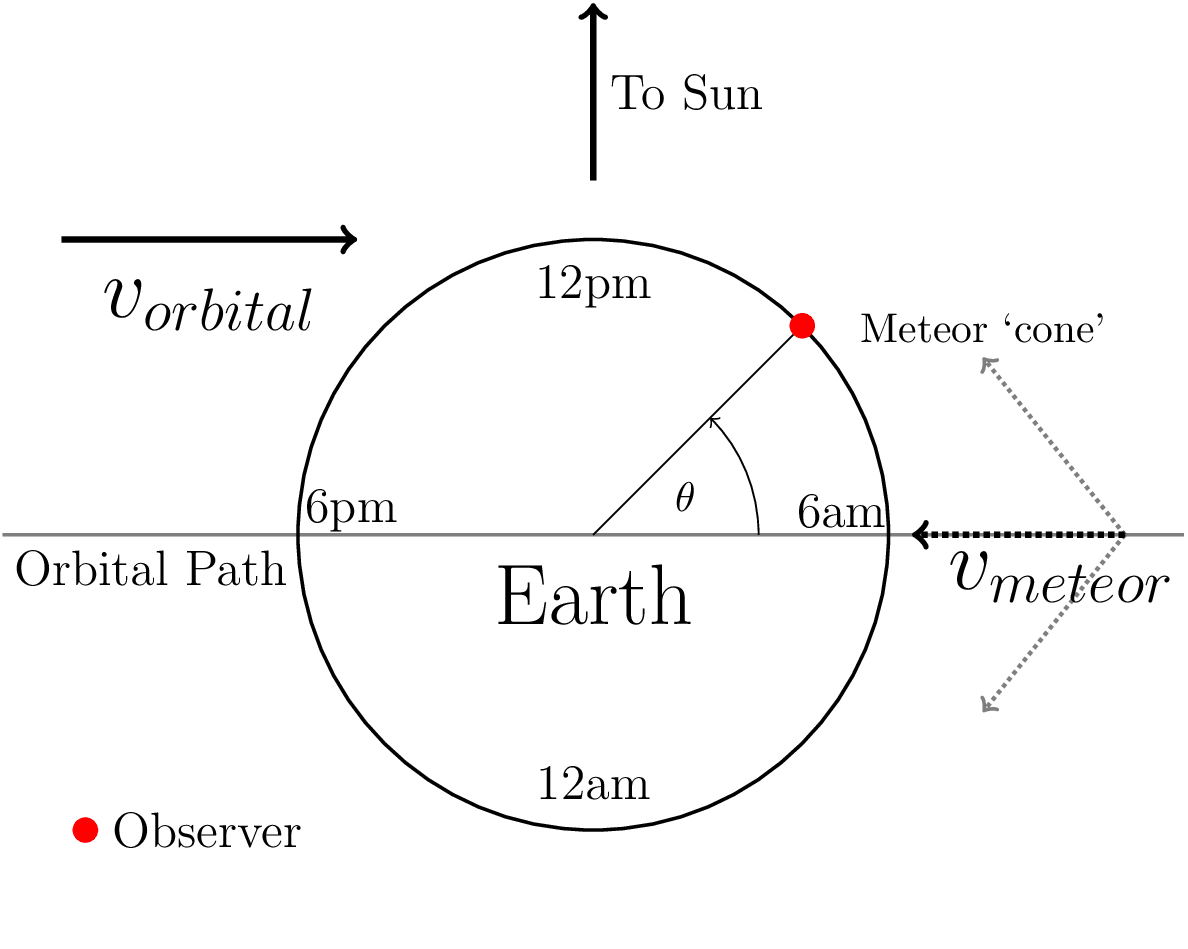
\includegraphics[width=\linewidth]{diagram}
	\end{frame}
	
	\begin{frame}
		\centering
		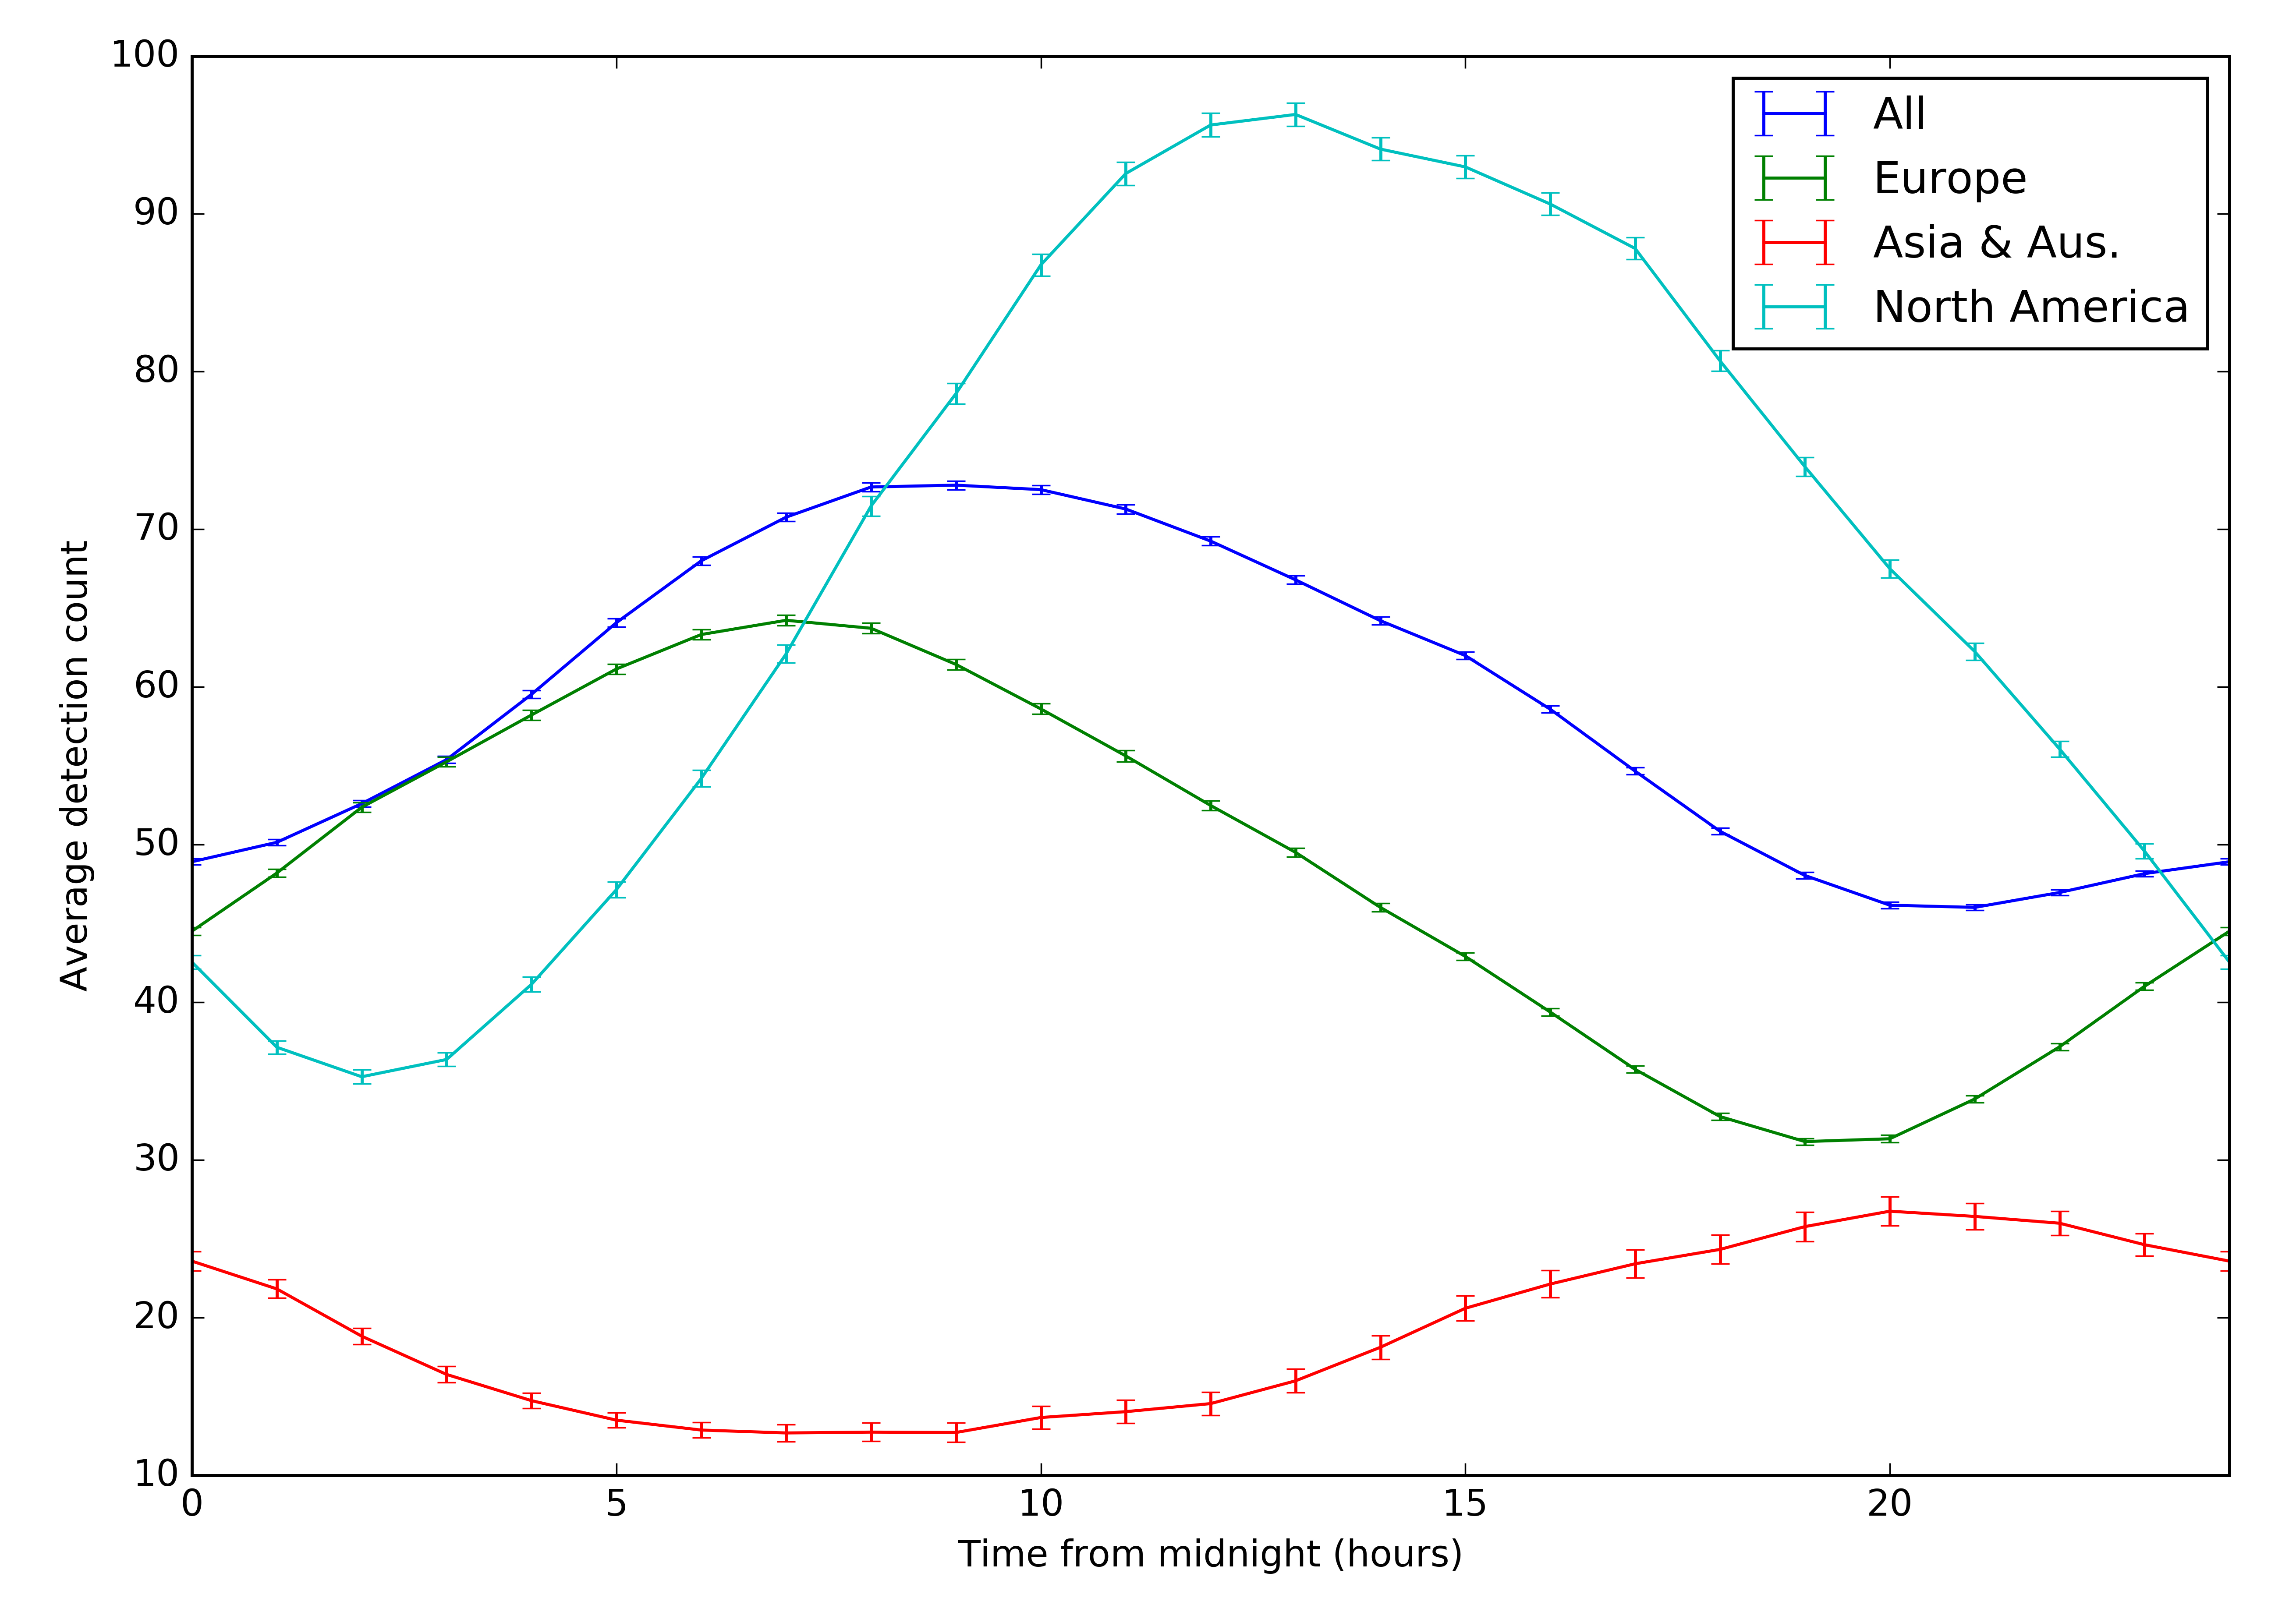
\includegraphics[width=\linewidth]{all_shifts}
	\end{frame}

	\begin{frame}
		\centering
		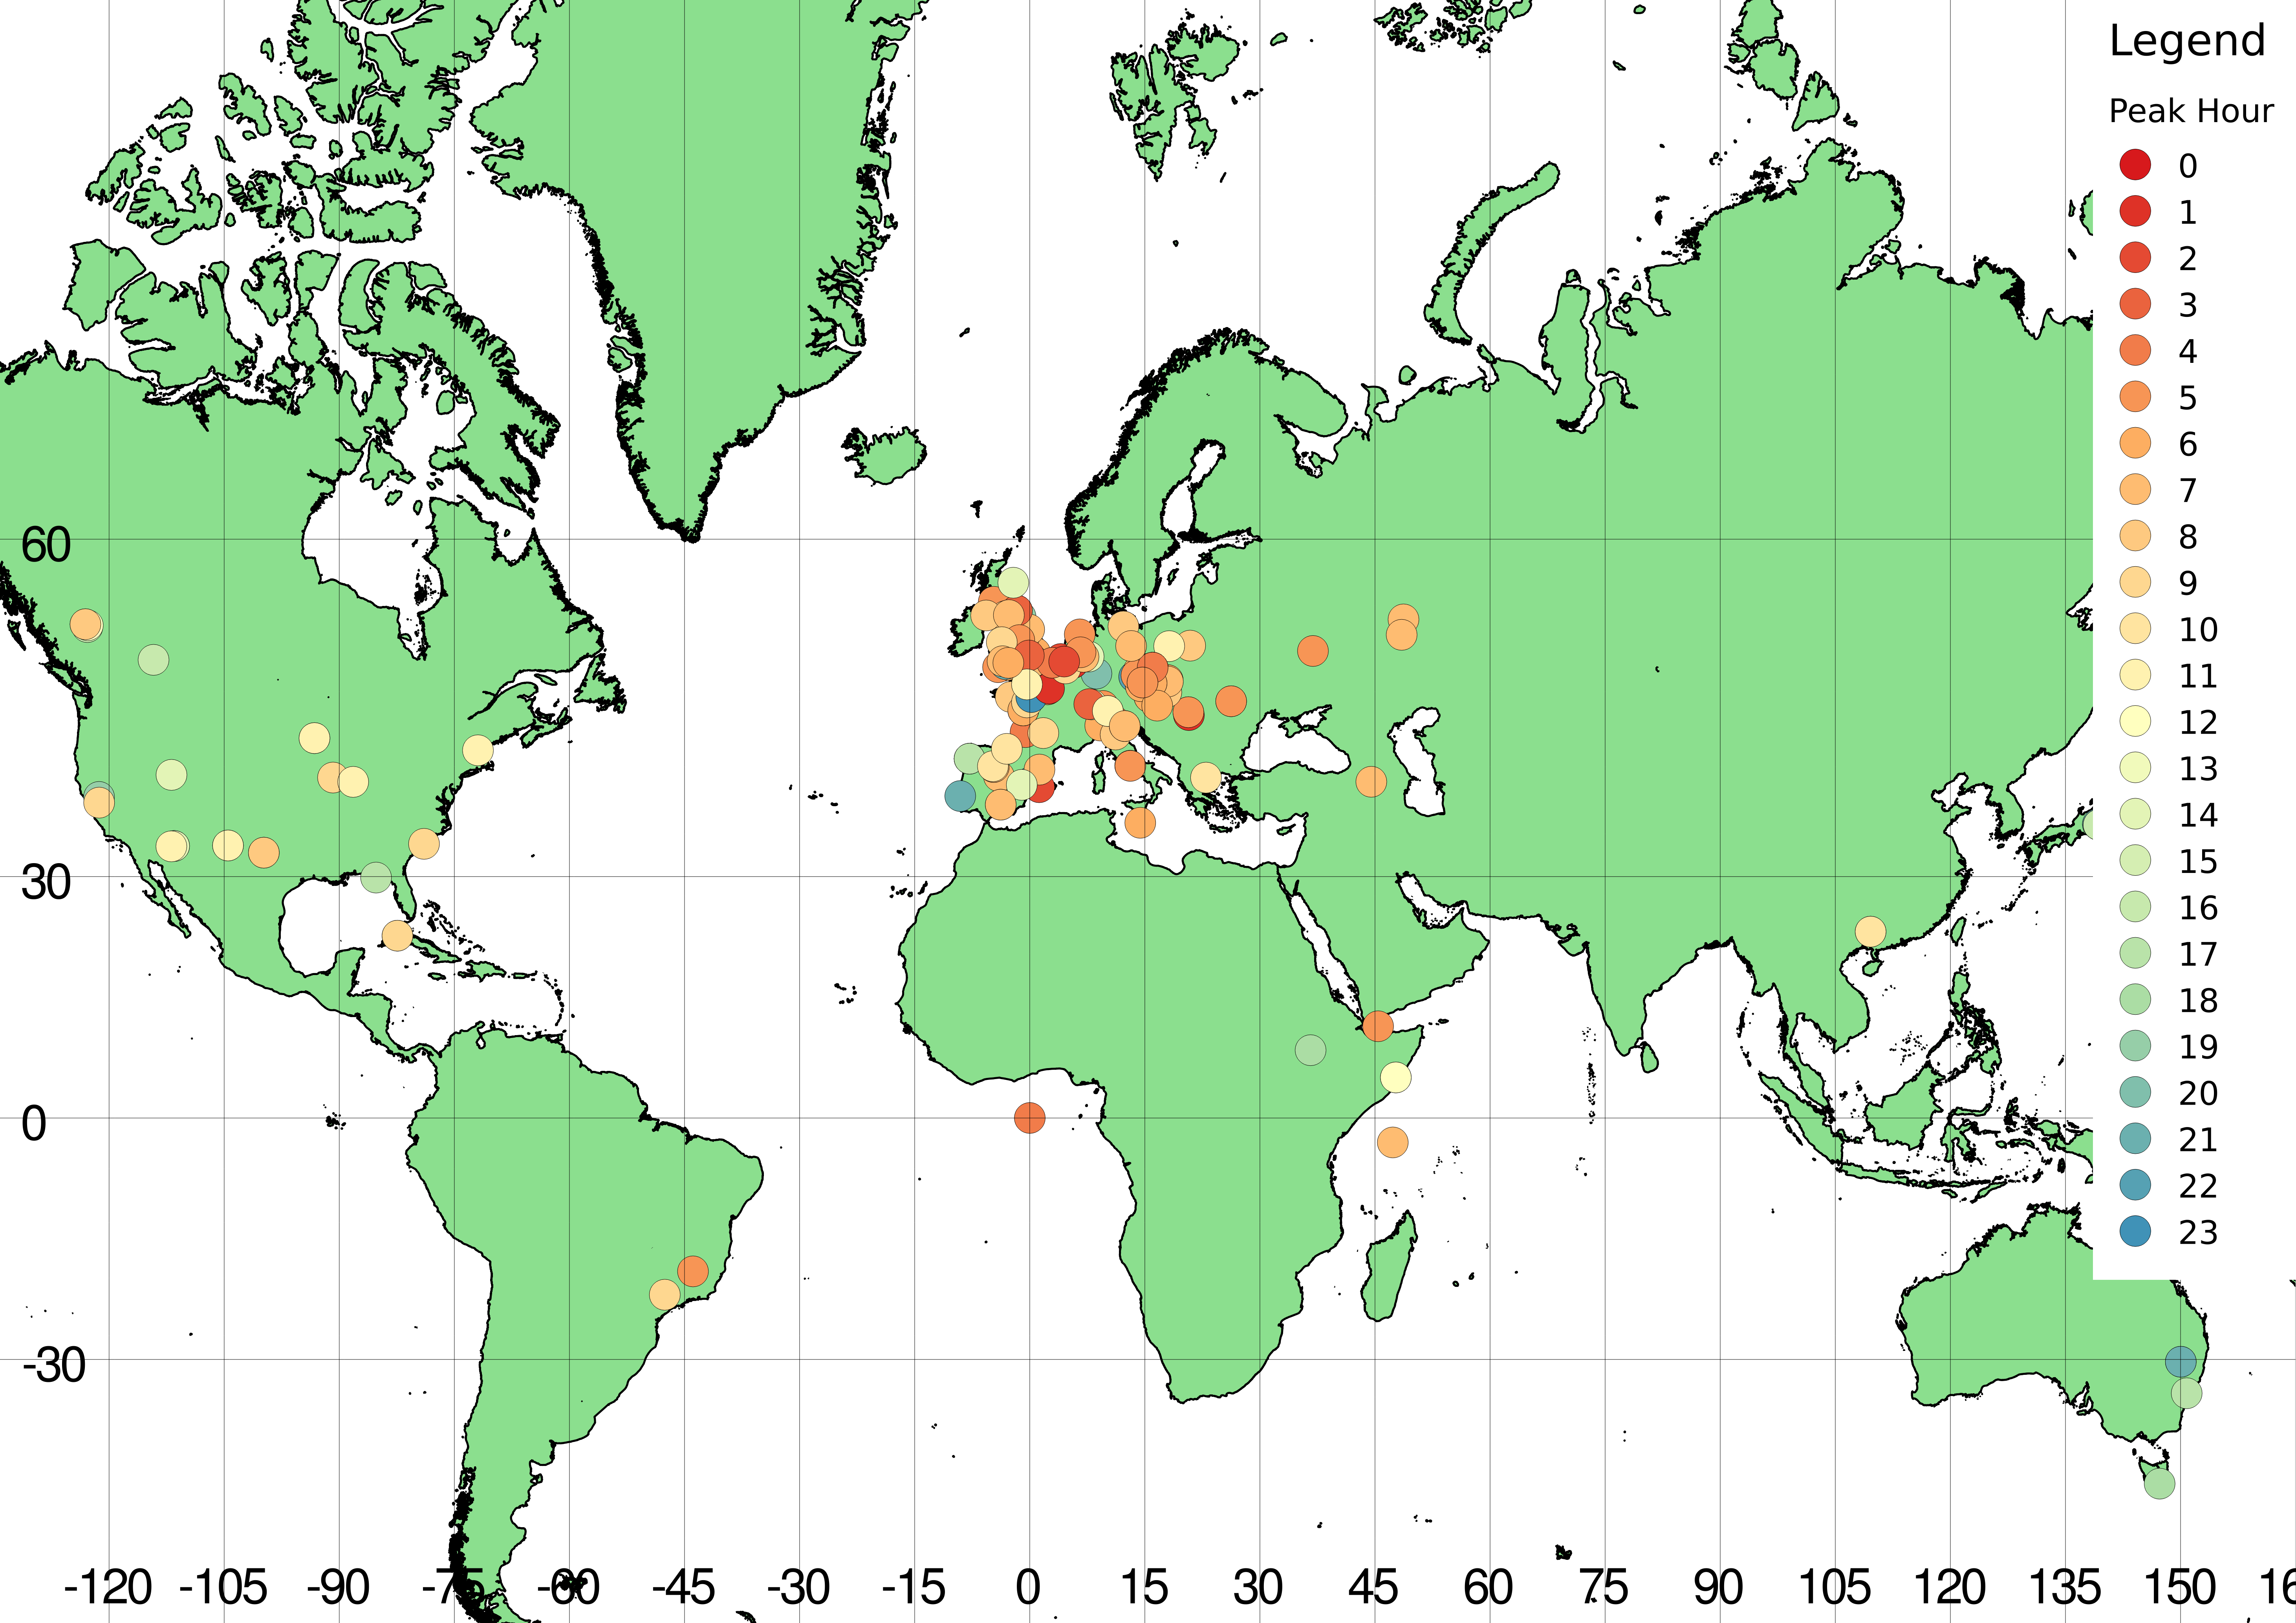
\includegraphics[width=\linewidth]{peak_qgis}
	\end{frame}
	
	\begin{frame}
		\centering
		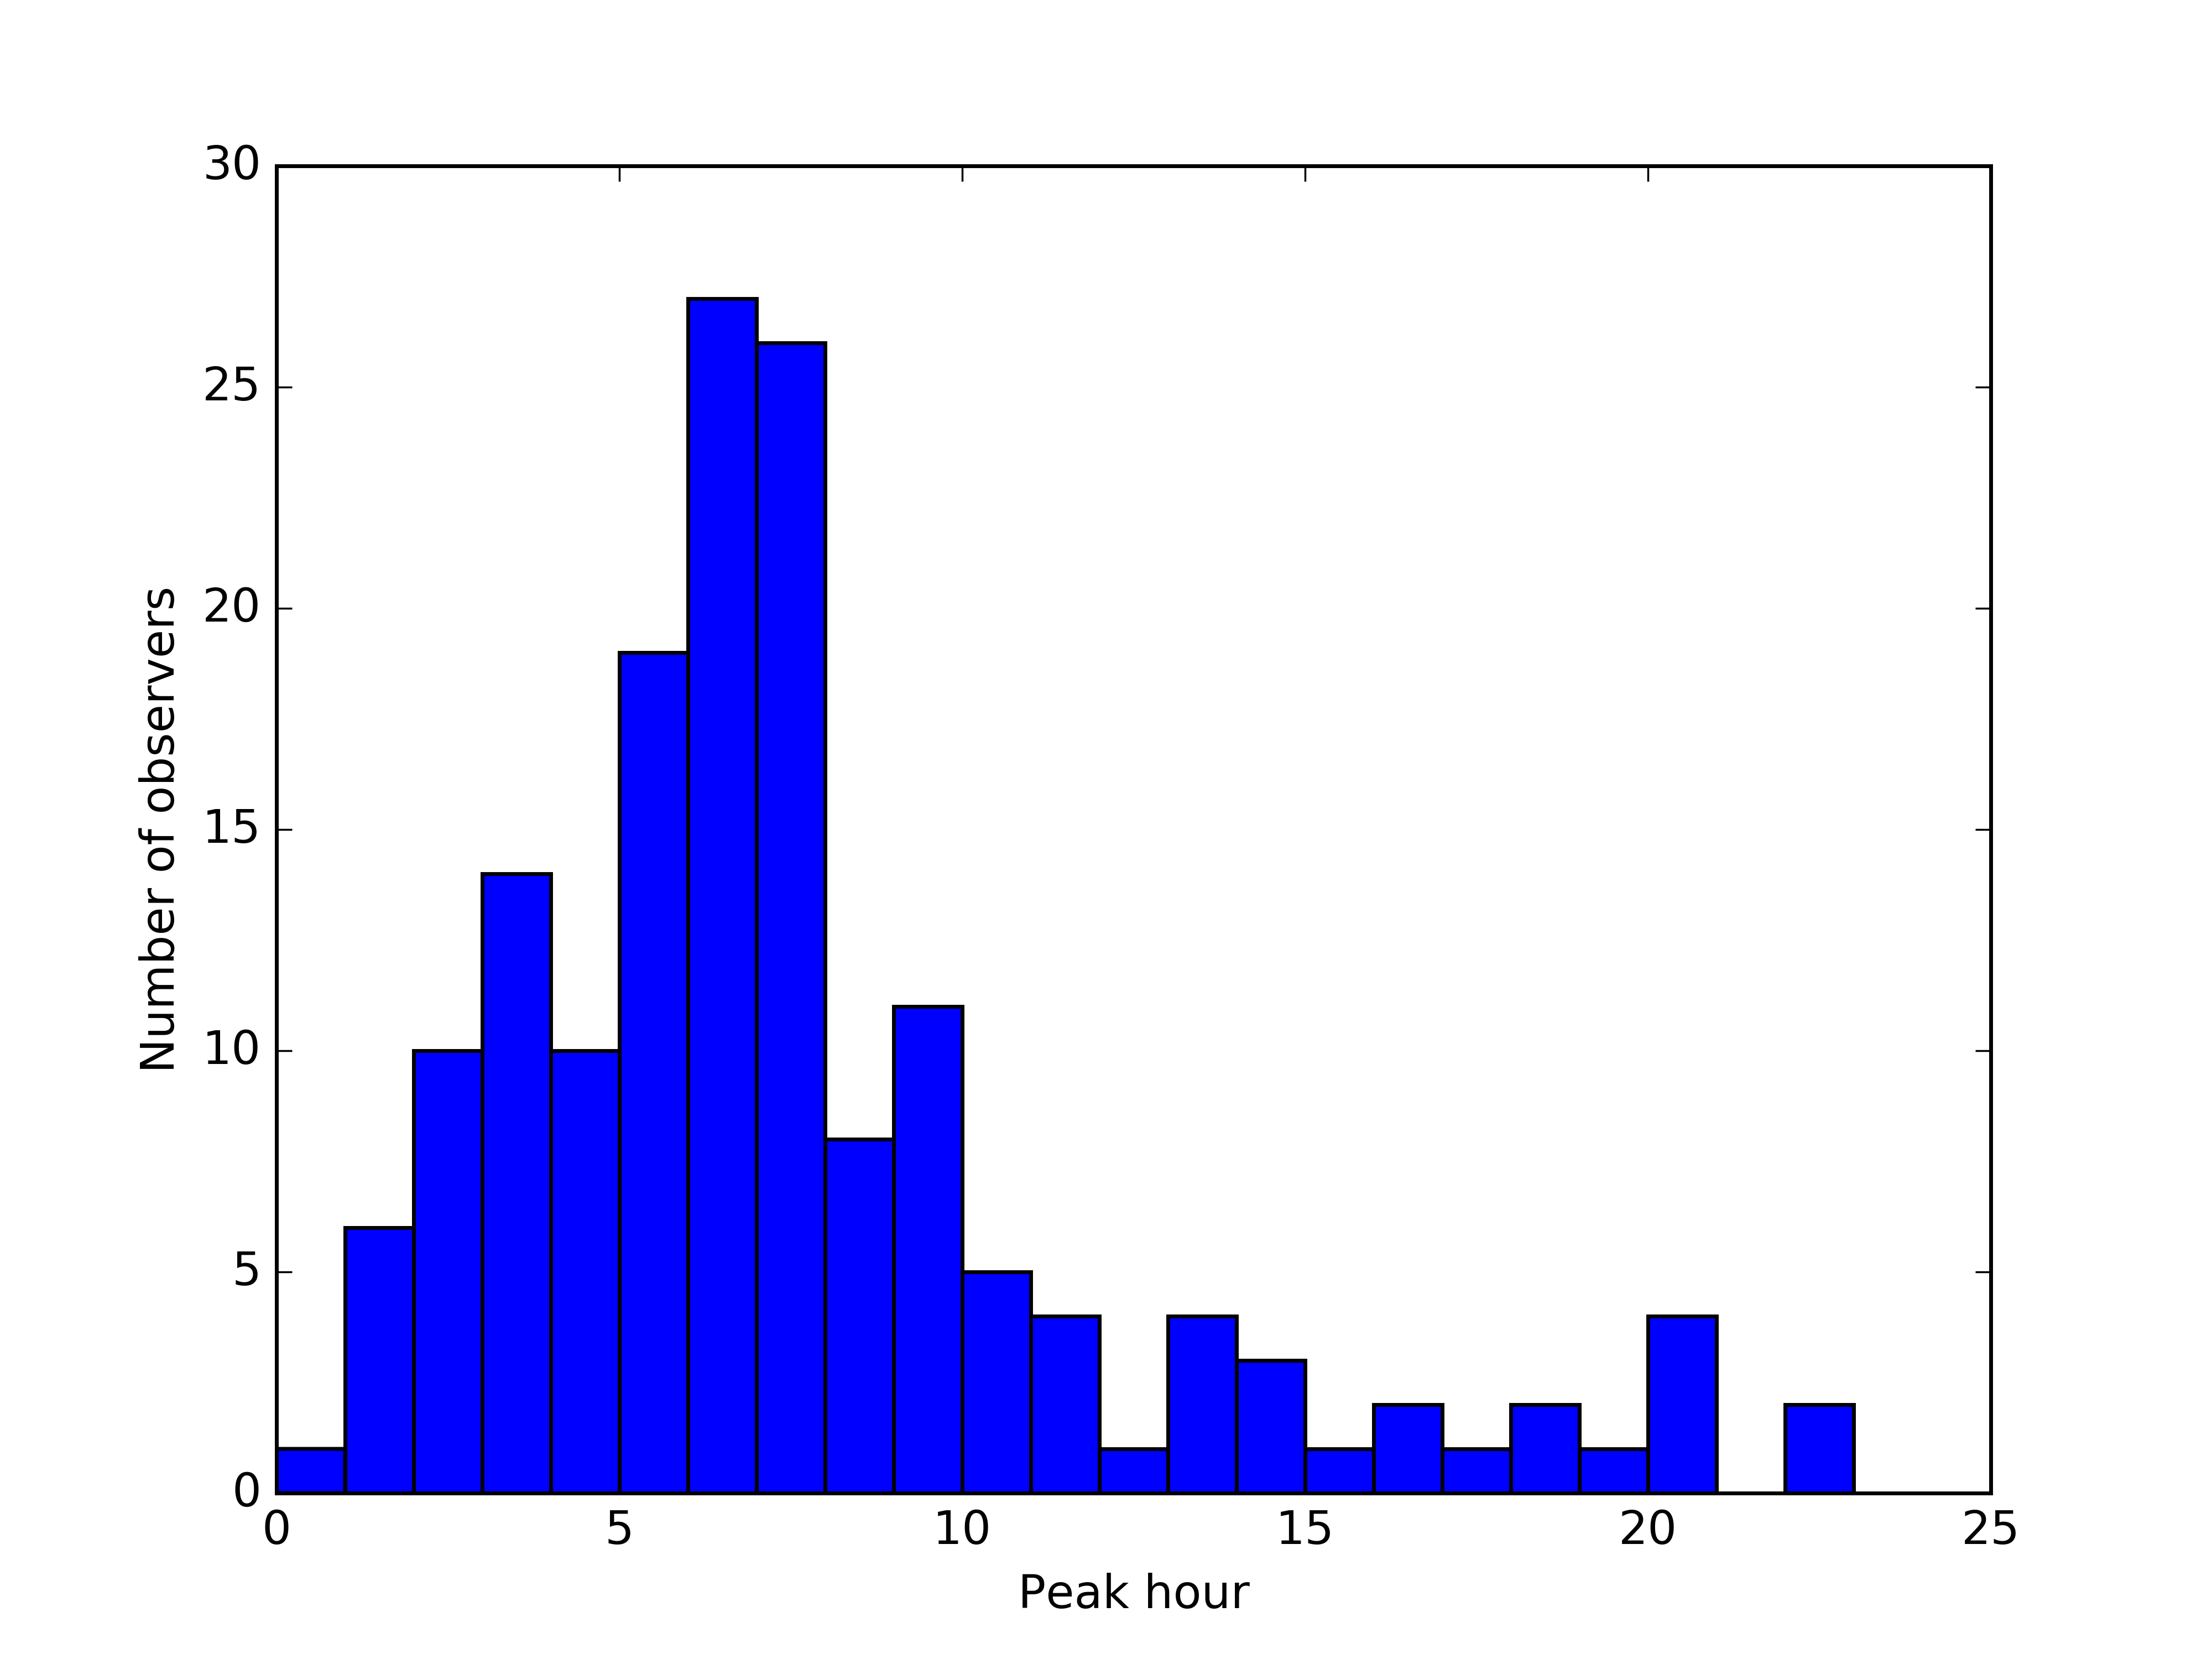
\includegraphics[width=\linewidth]{hist}
	\end{frame}
	
	\begin{frame}
		\centering
		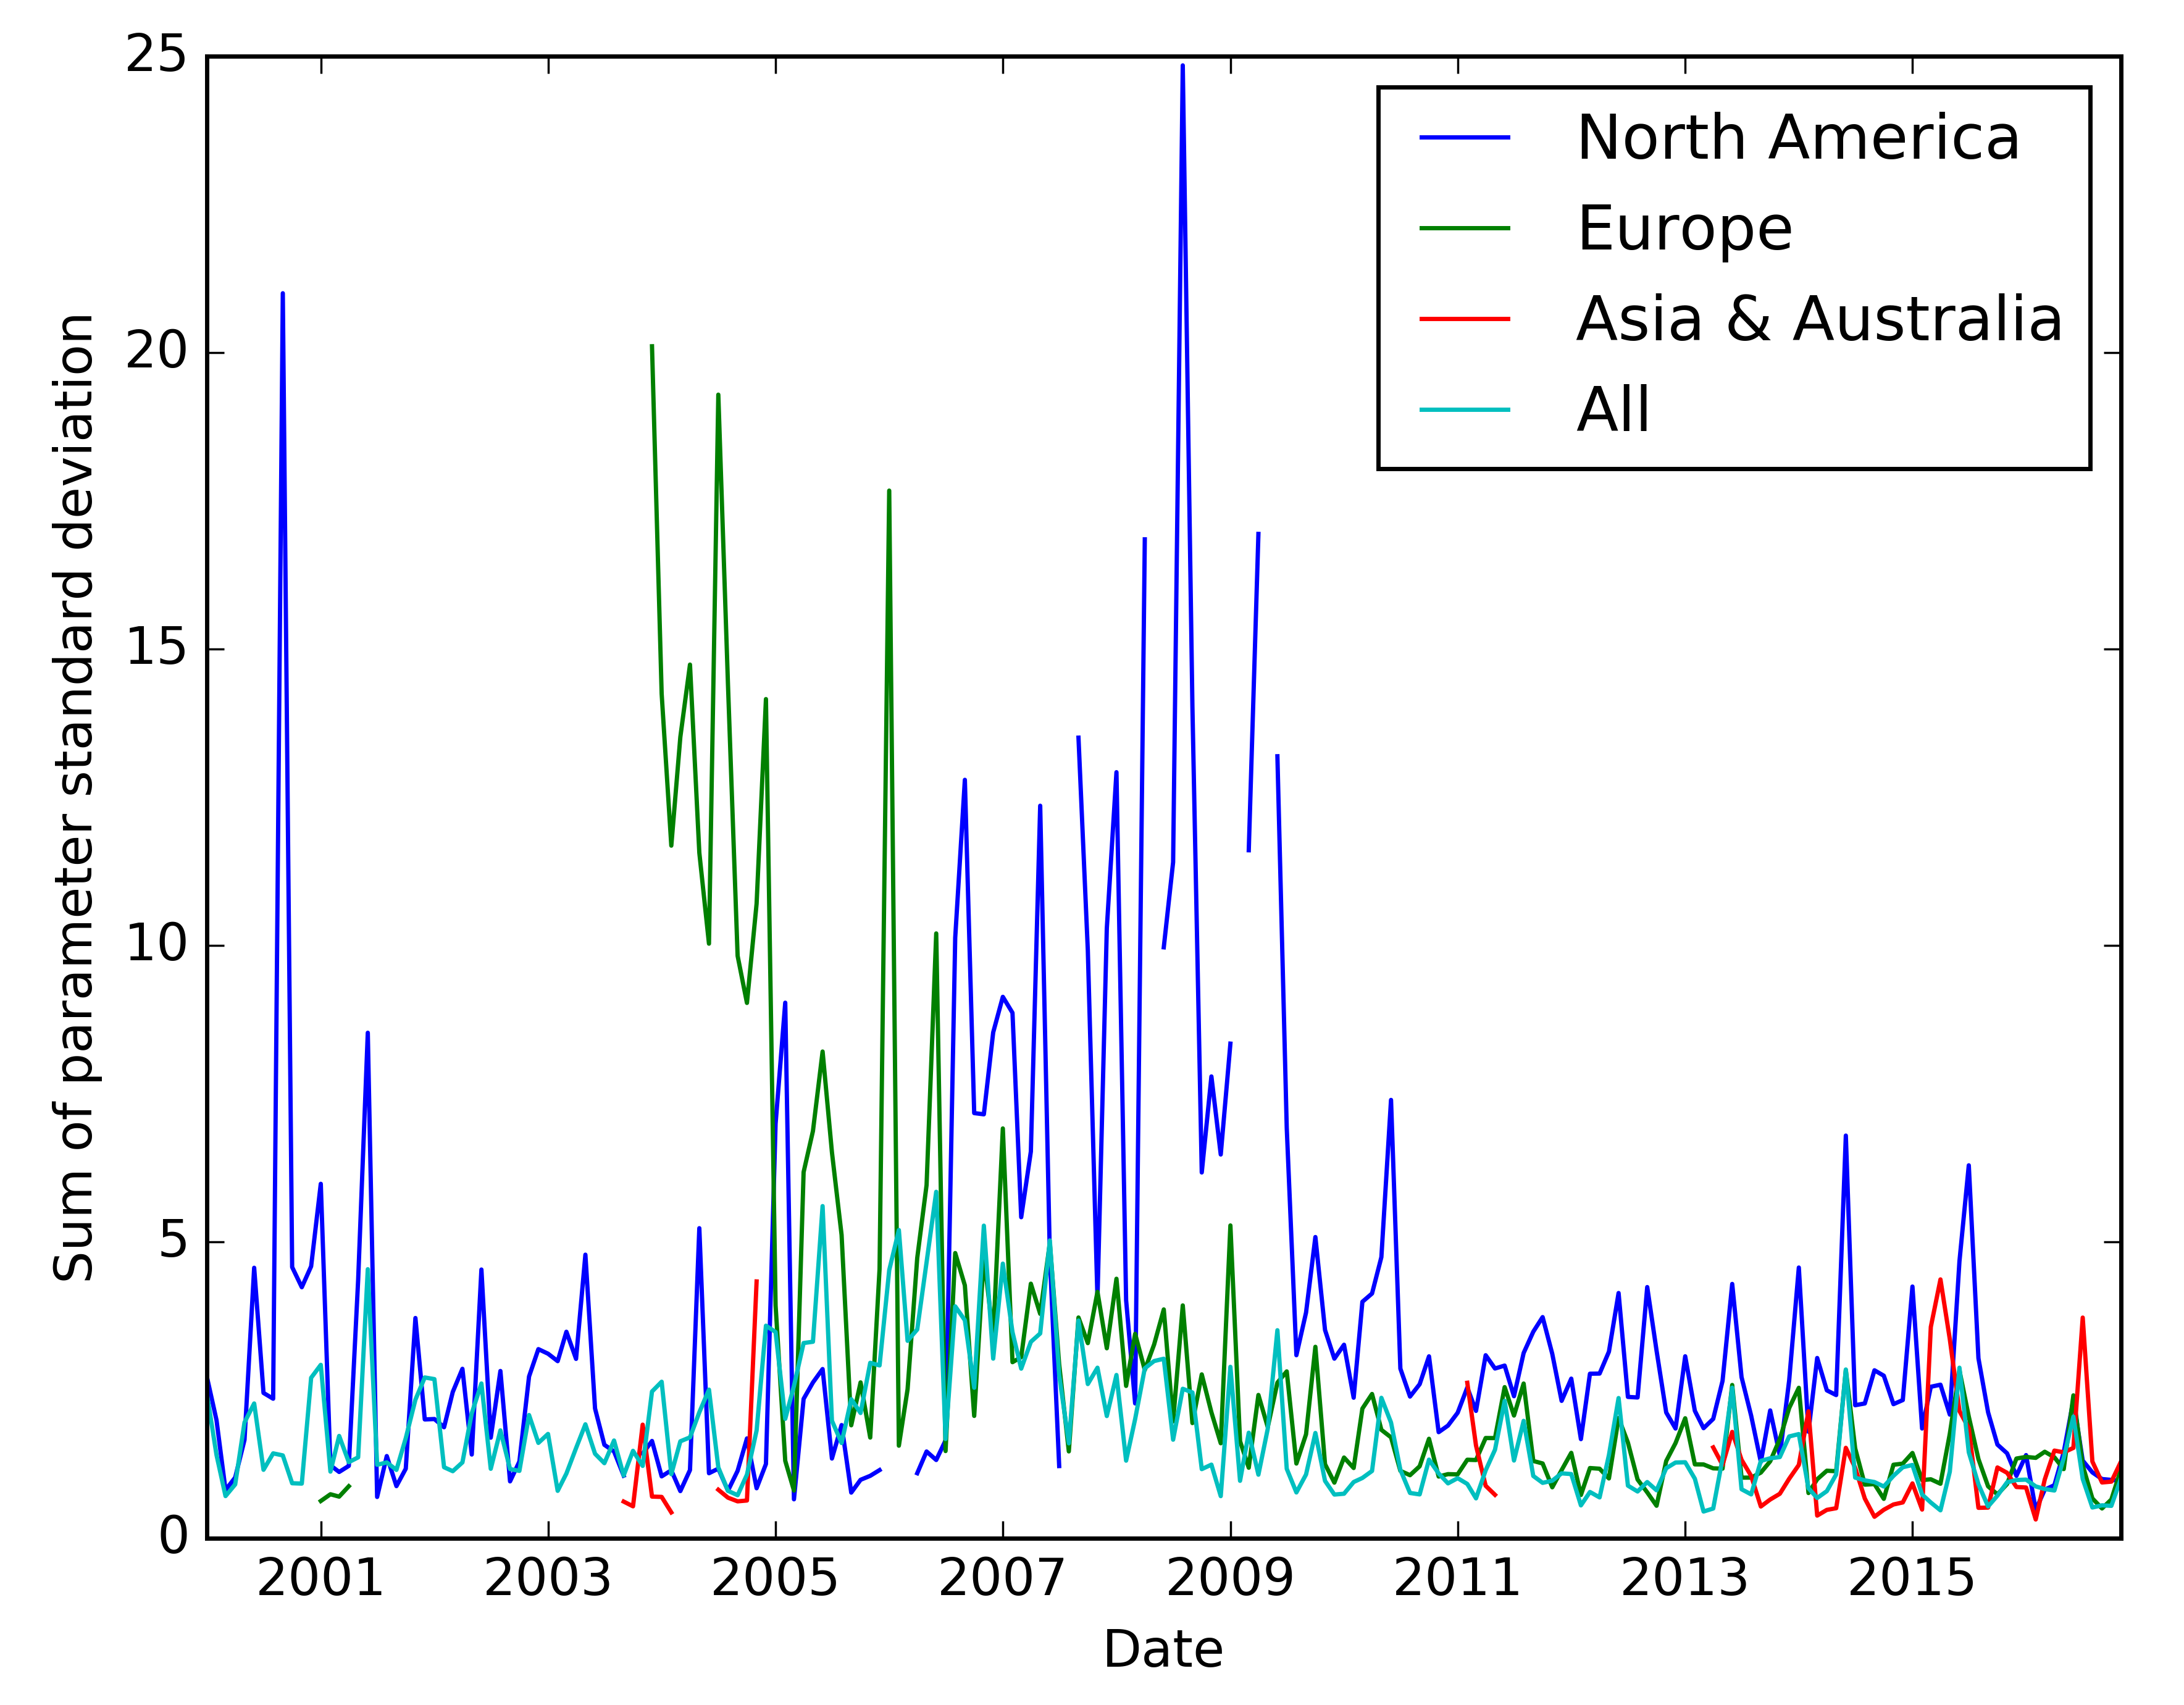
\includegraphics[width=\linewidth]{COMBINEDfit}
	\end{frame}
	
	\section{Temporal variation}
	\begin{frame}
		\centering
		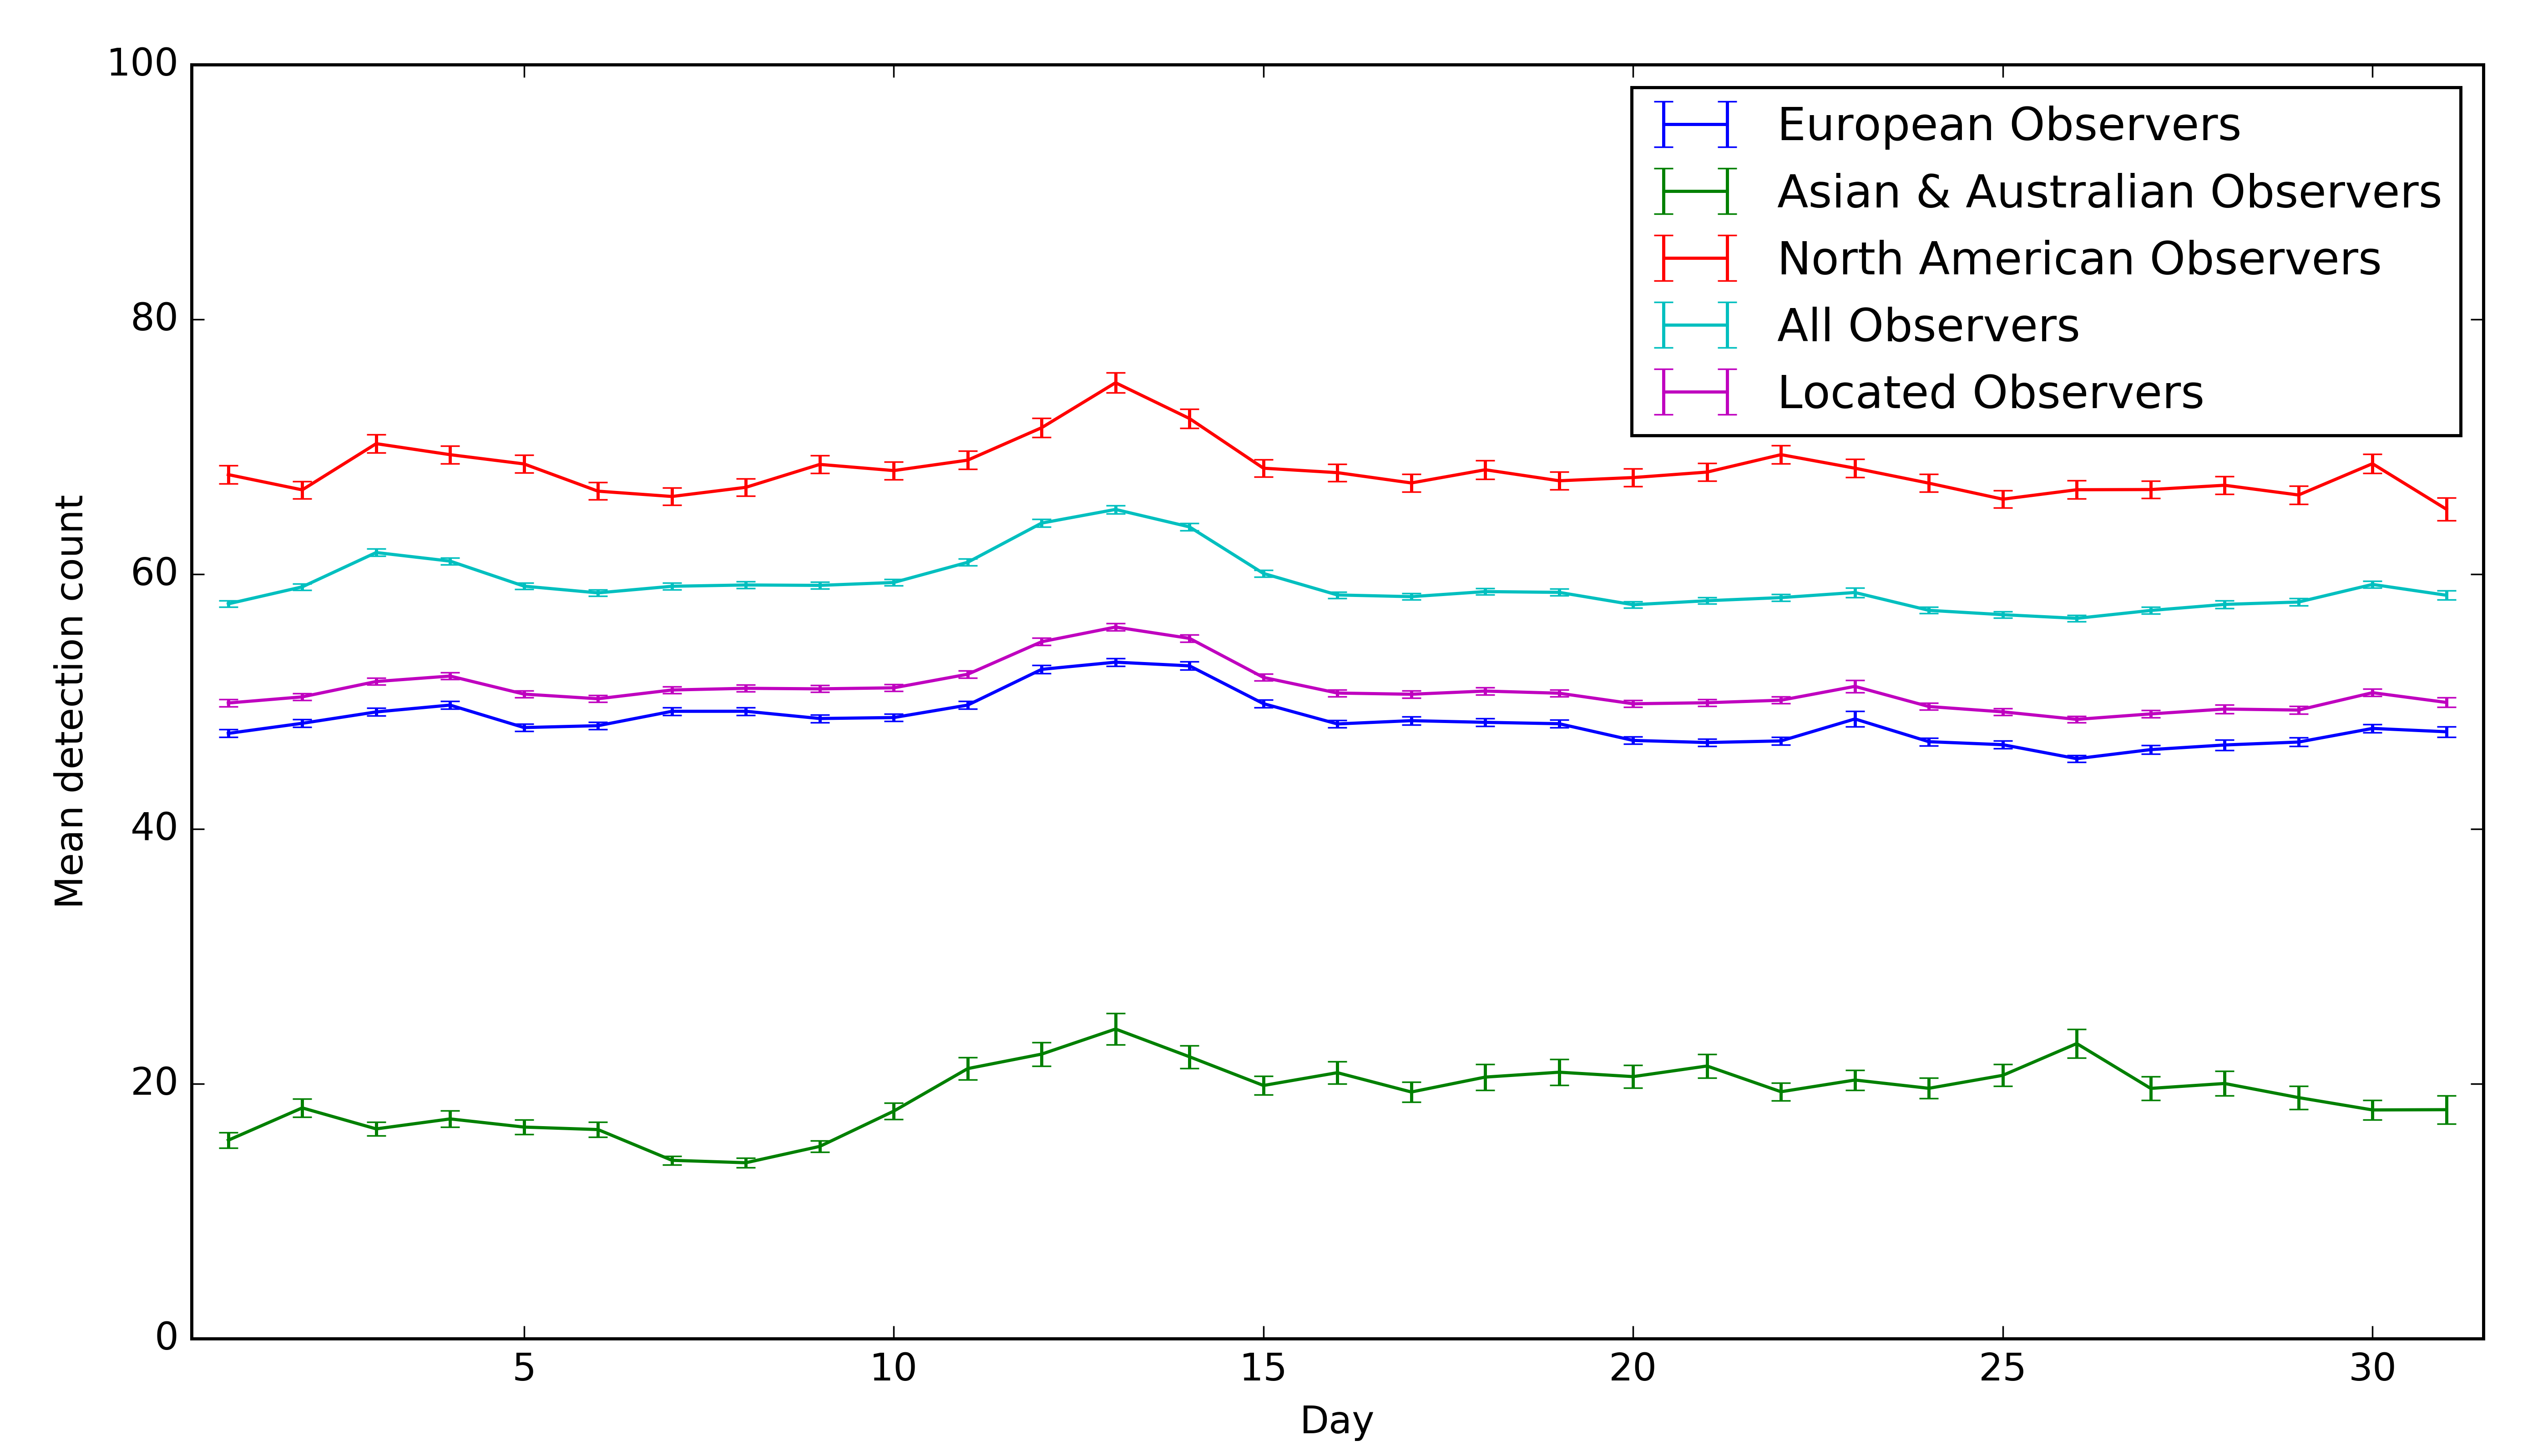
\includegraphics[width=\linewidth]{Dcombined}
	\end{frame}

	\begin{frame}
		\centering
		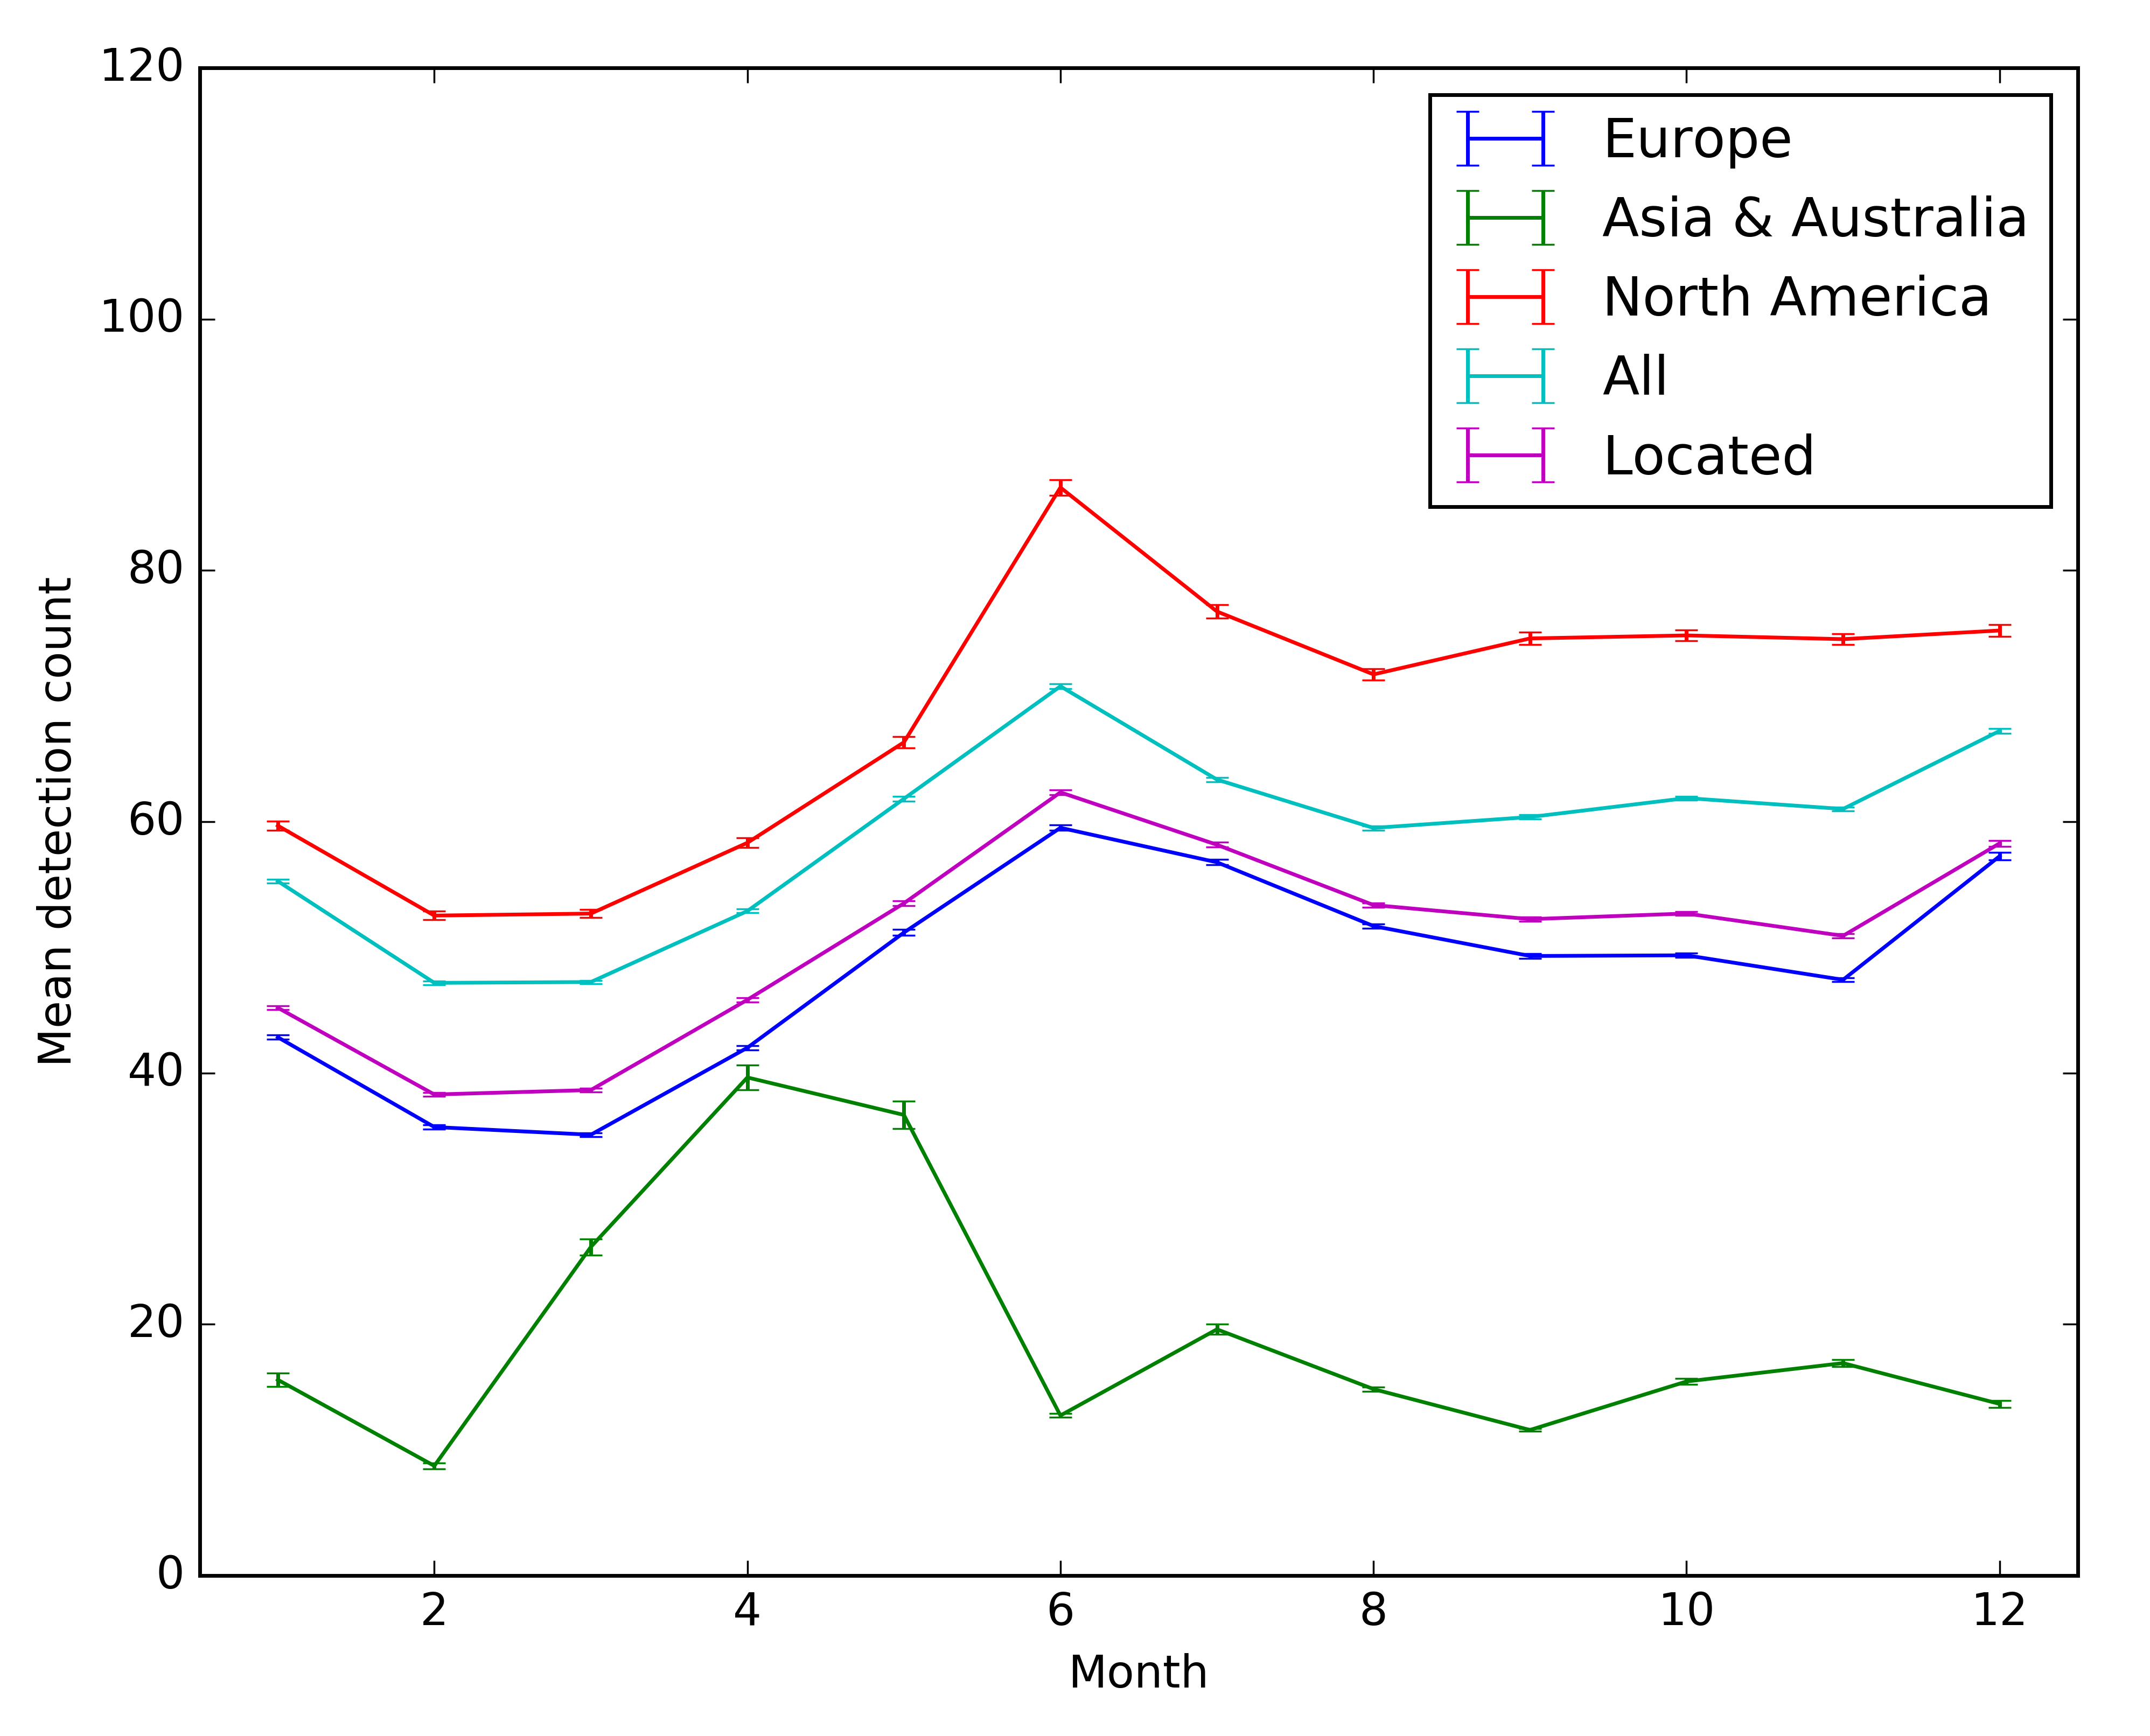
\includegraphics[width=\linewidth]{Mcombined}	
	\end{frame}

	\begin{frame}
		\centering
		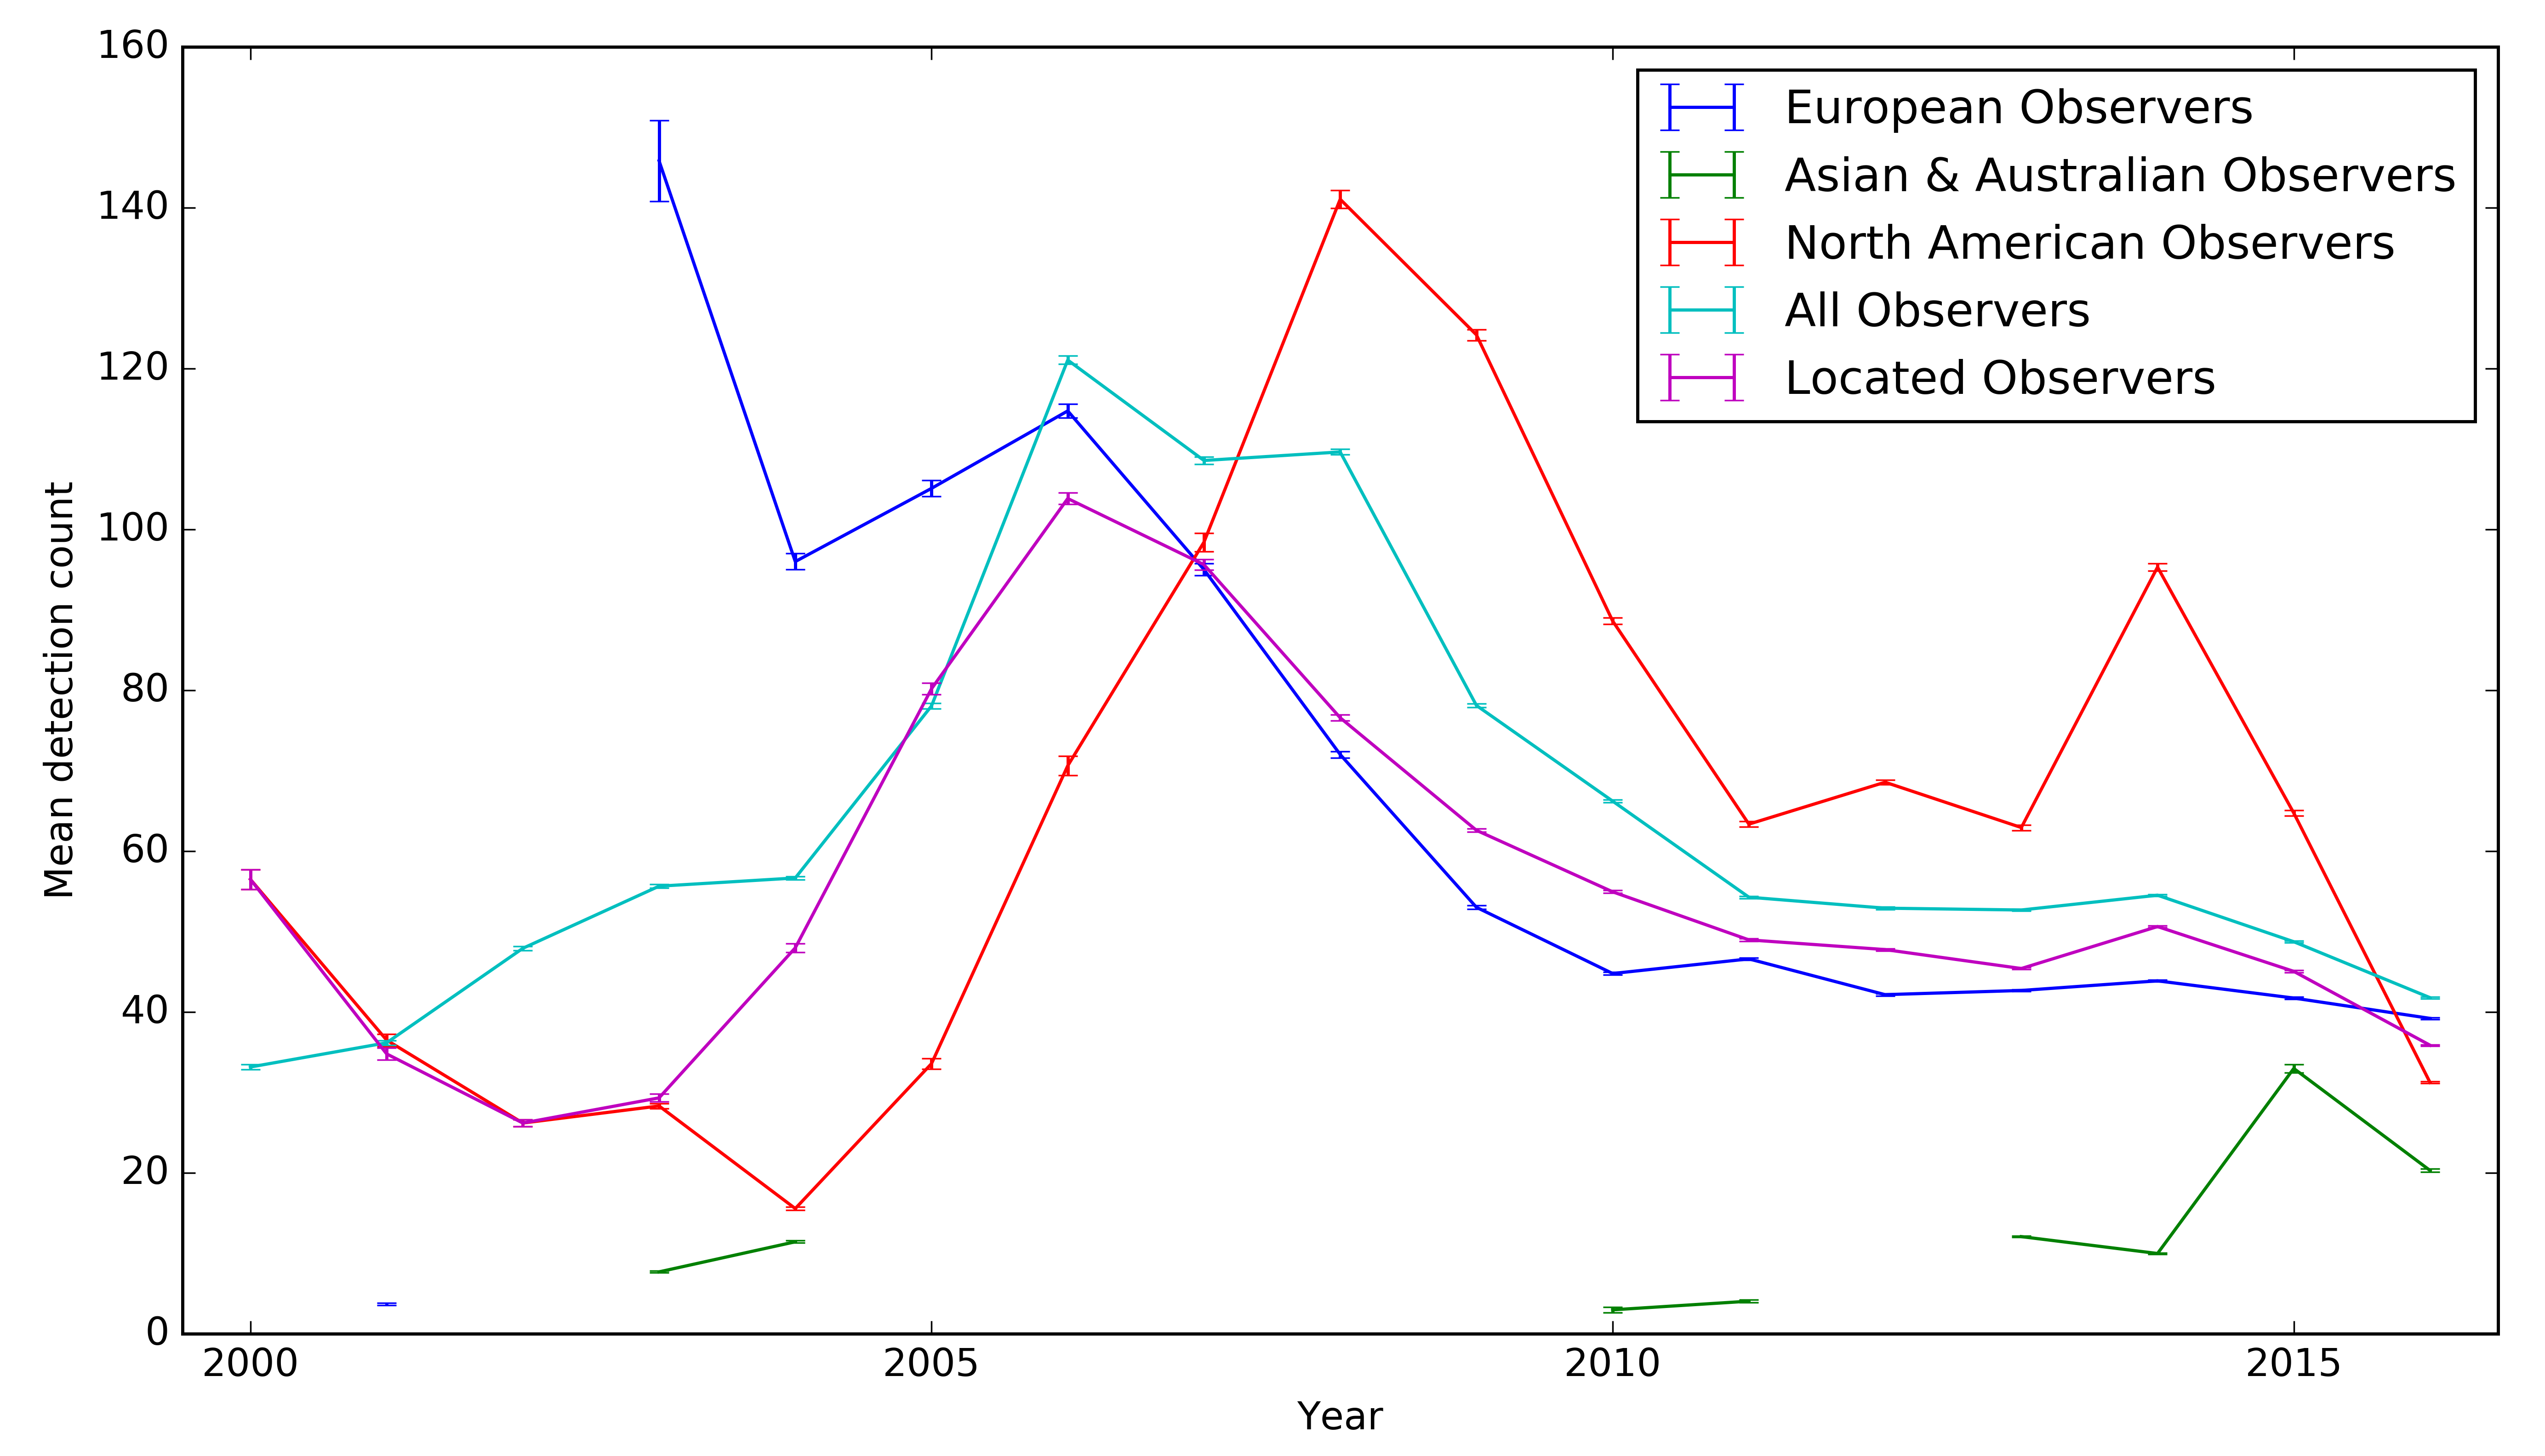
\includegraphics[width=\linewidth]{Ycombined}
	\end{frame}
	
	\begin{frame}
		\centering
		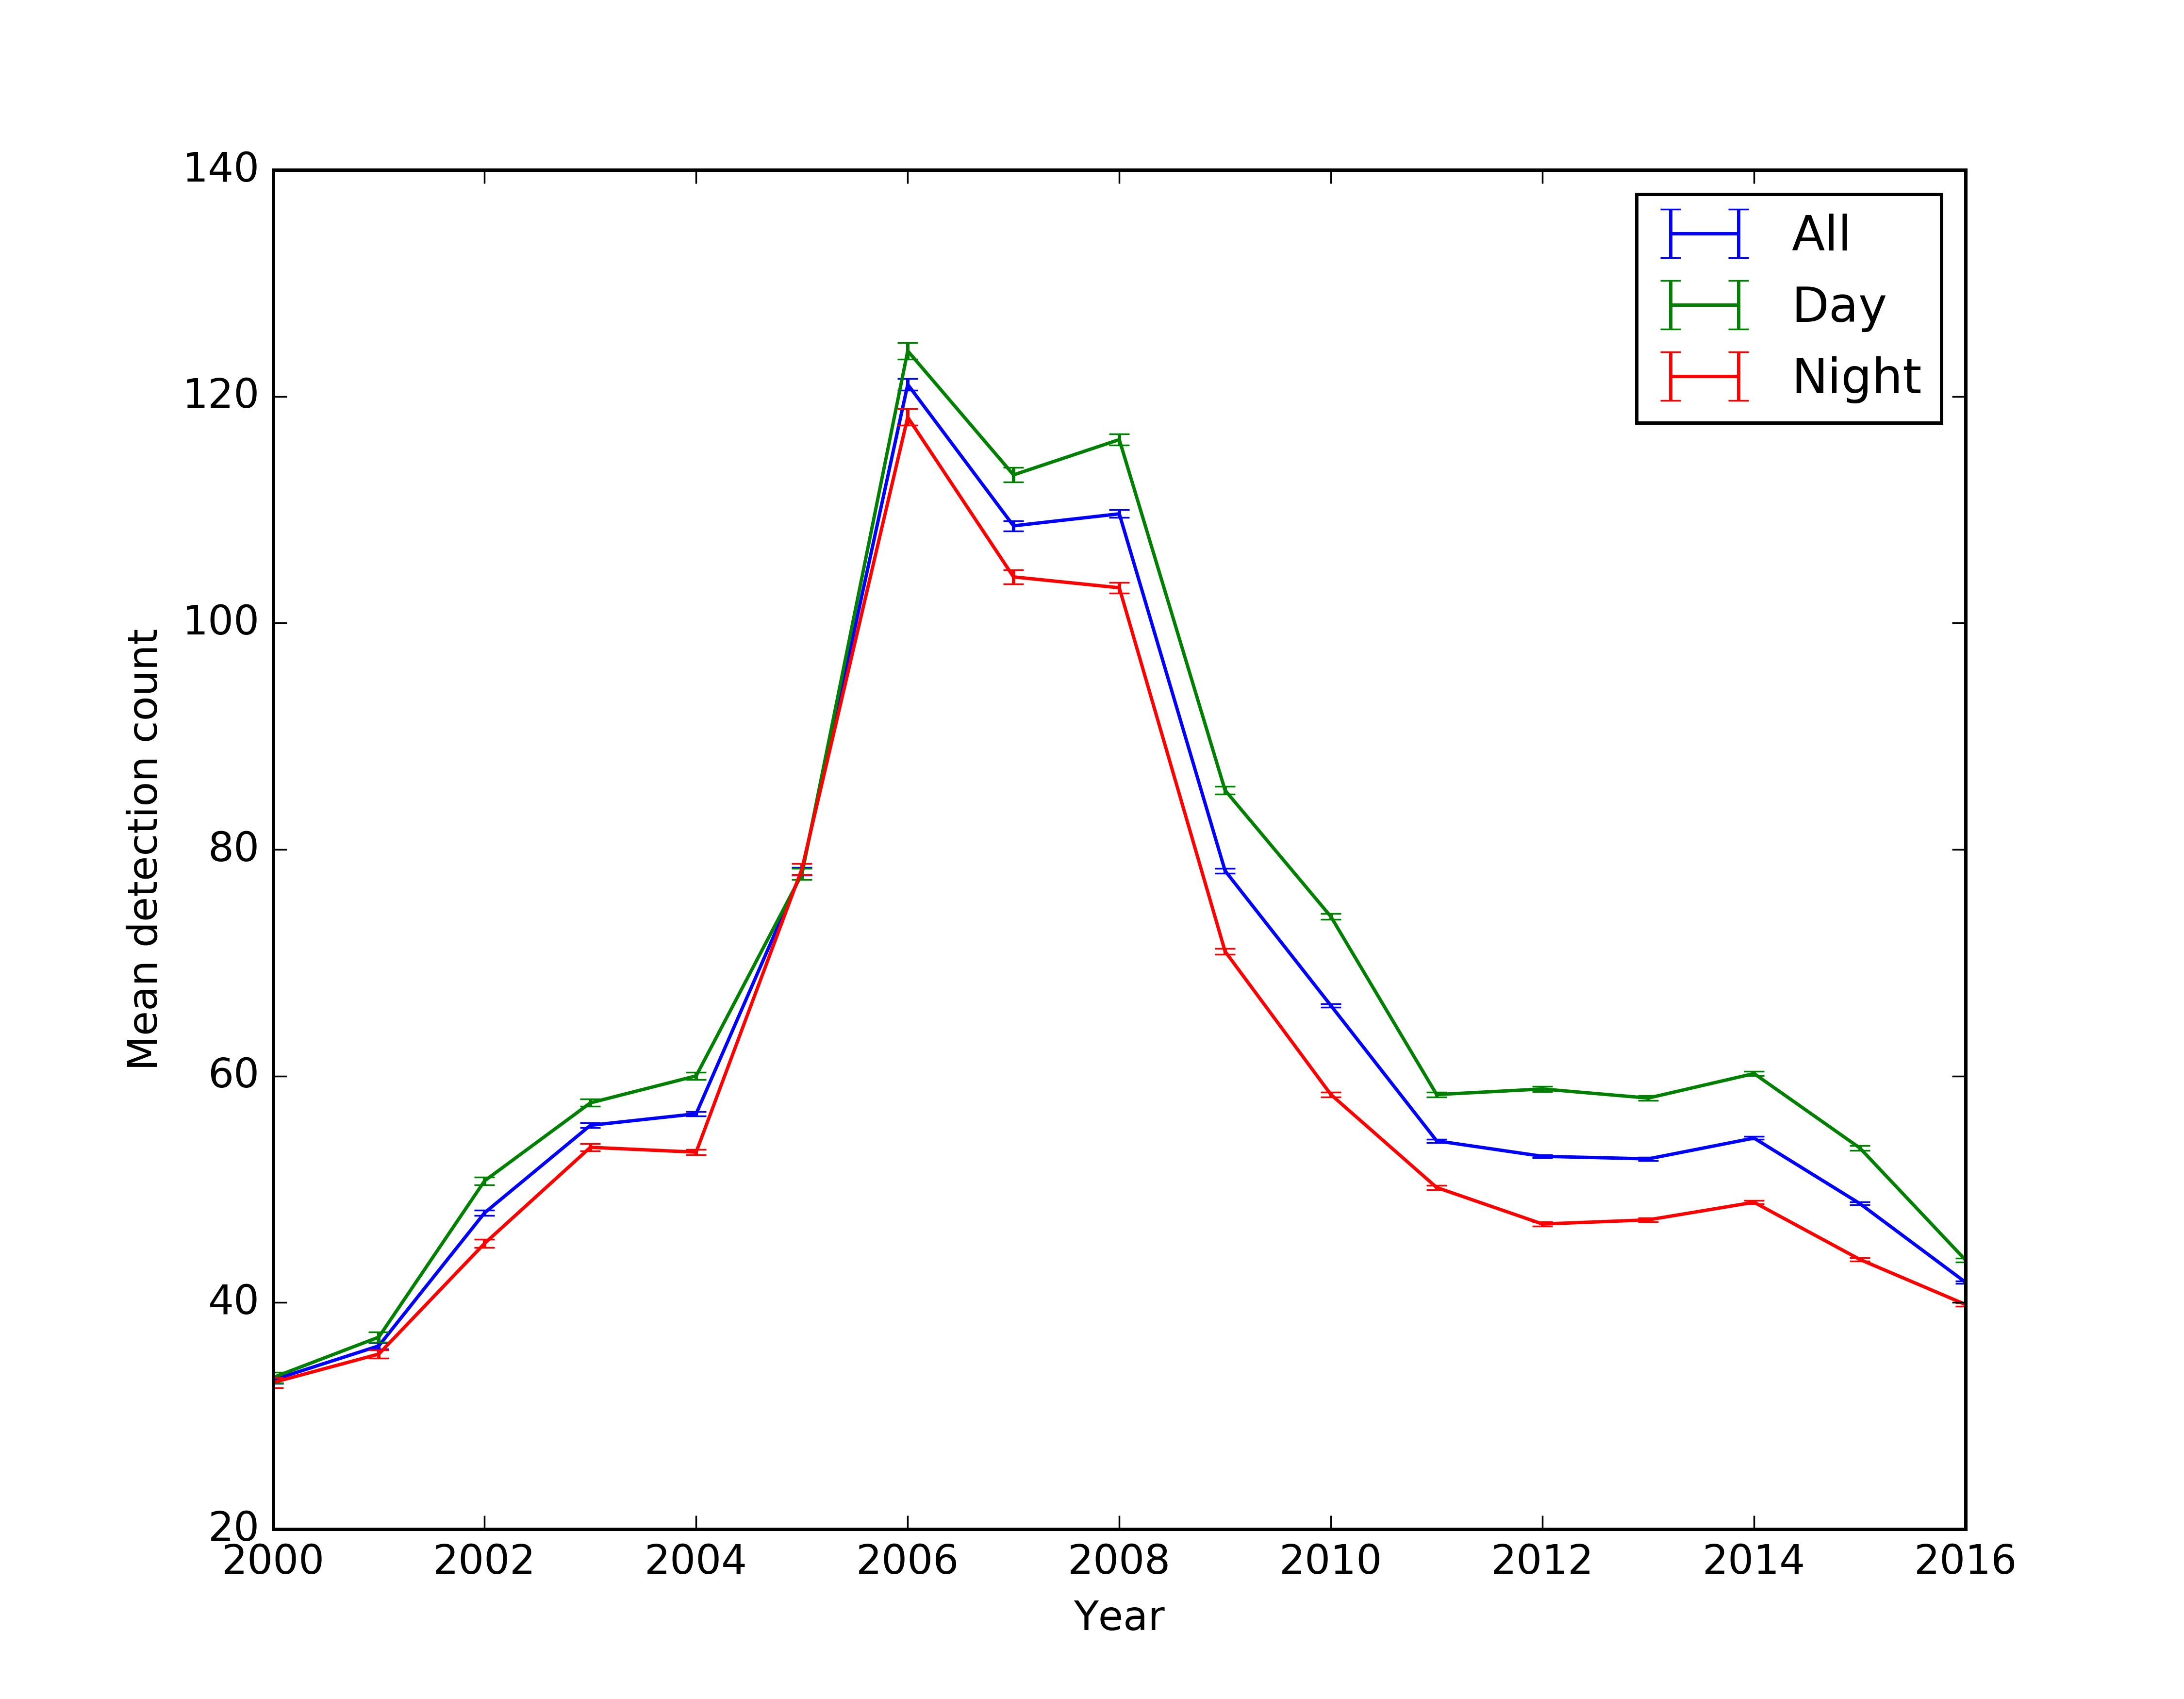
\includegraphics[width=\linewidth]{YAllcombined}
	\end{frame}

	\section{Zenithal hourly rate}
	\begin{frame}
		\[ {ZHR} = \frac{\overline{HR} \cdot F \cdot r^{6.5-{m}}}{\sin \left( h \right)} \]
		$\overline{HR} =$ number of detected meteors in an hour\\
		$F =$ correction for \% of sky obstructed\\
		$r =$ population index\\
		$m =$ limiting magnitude\\
		$h =$ angular radiant height
	\end{frame}

	\begin{frame}
		\[ {ZHR} = \frac{N - r}{\left( \frac{1}{2} + \frac{h}{2\pi} \right)}
		\cdot F \cdot M \]
		$h =$ angular radiant height\\
		$N =$ number of detected meteors in an hour\\
		$r =$ background hourly detection rate\\
		$F =$ correction for \% of sky obstructed\\
		$M =$ correction for limiting magnitude
	\end{frame}

	\begin{frame}
		\centering
		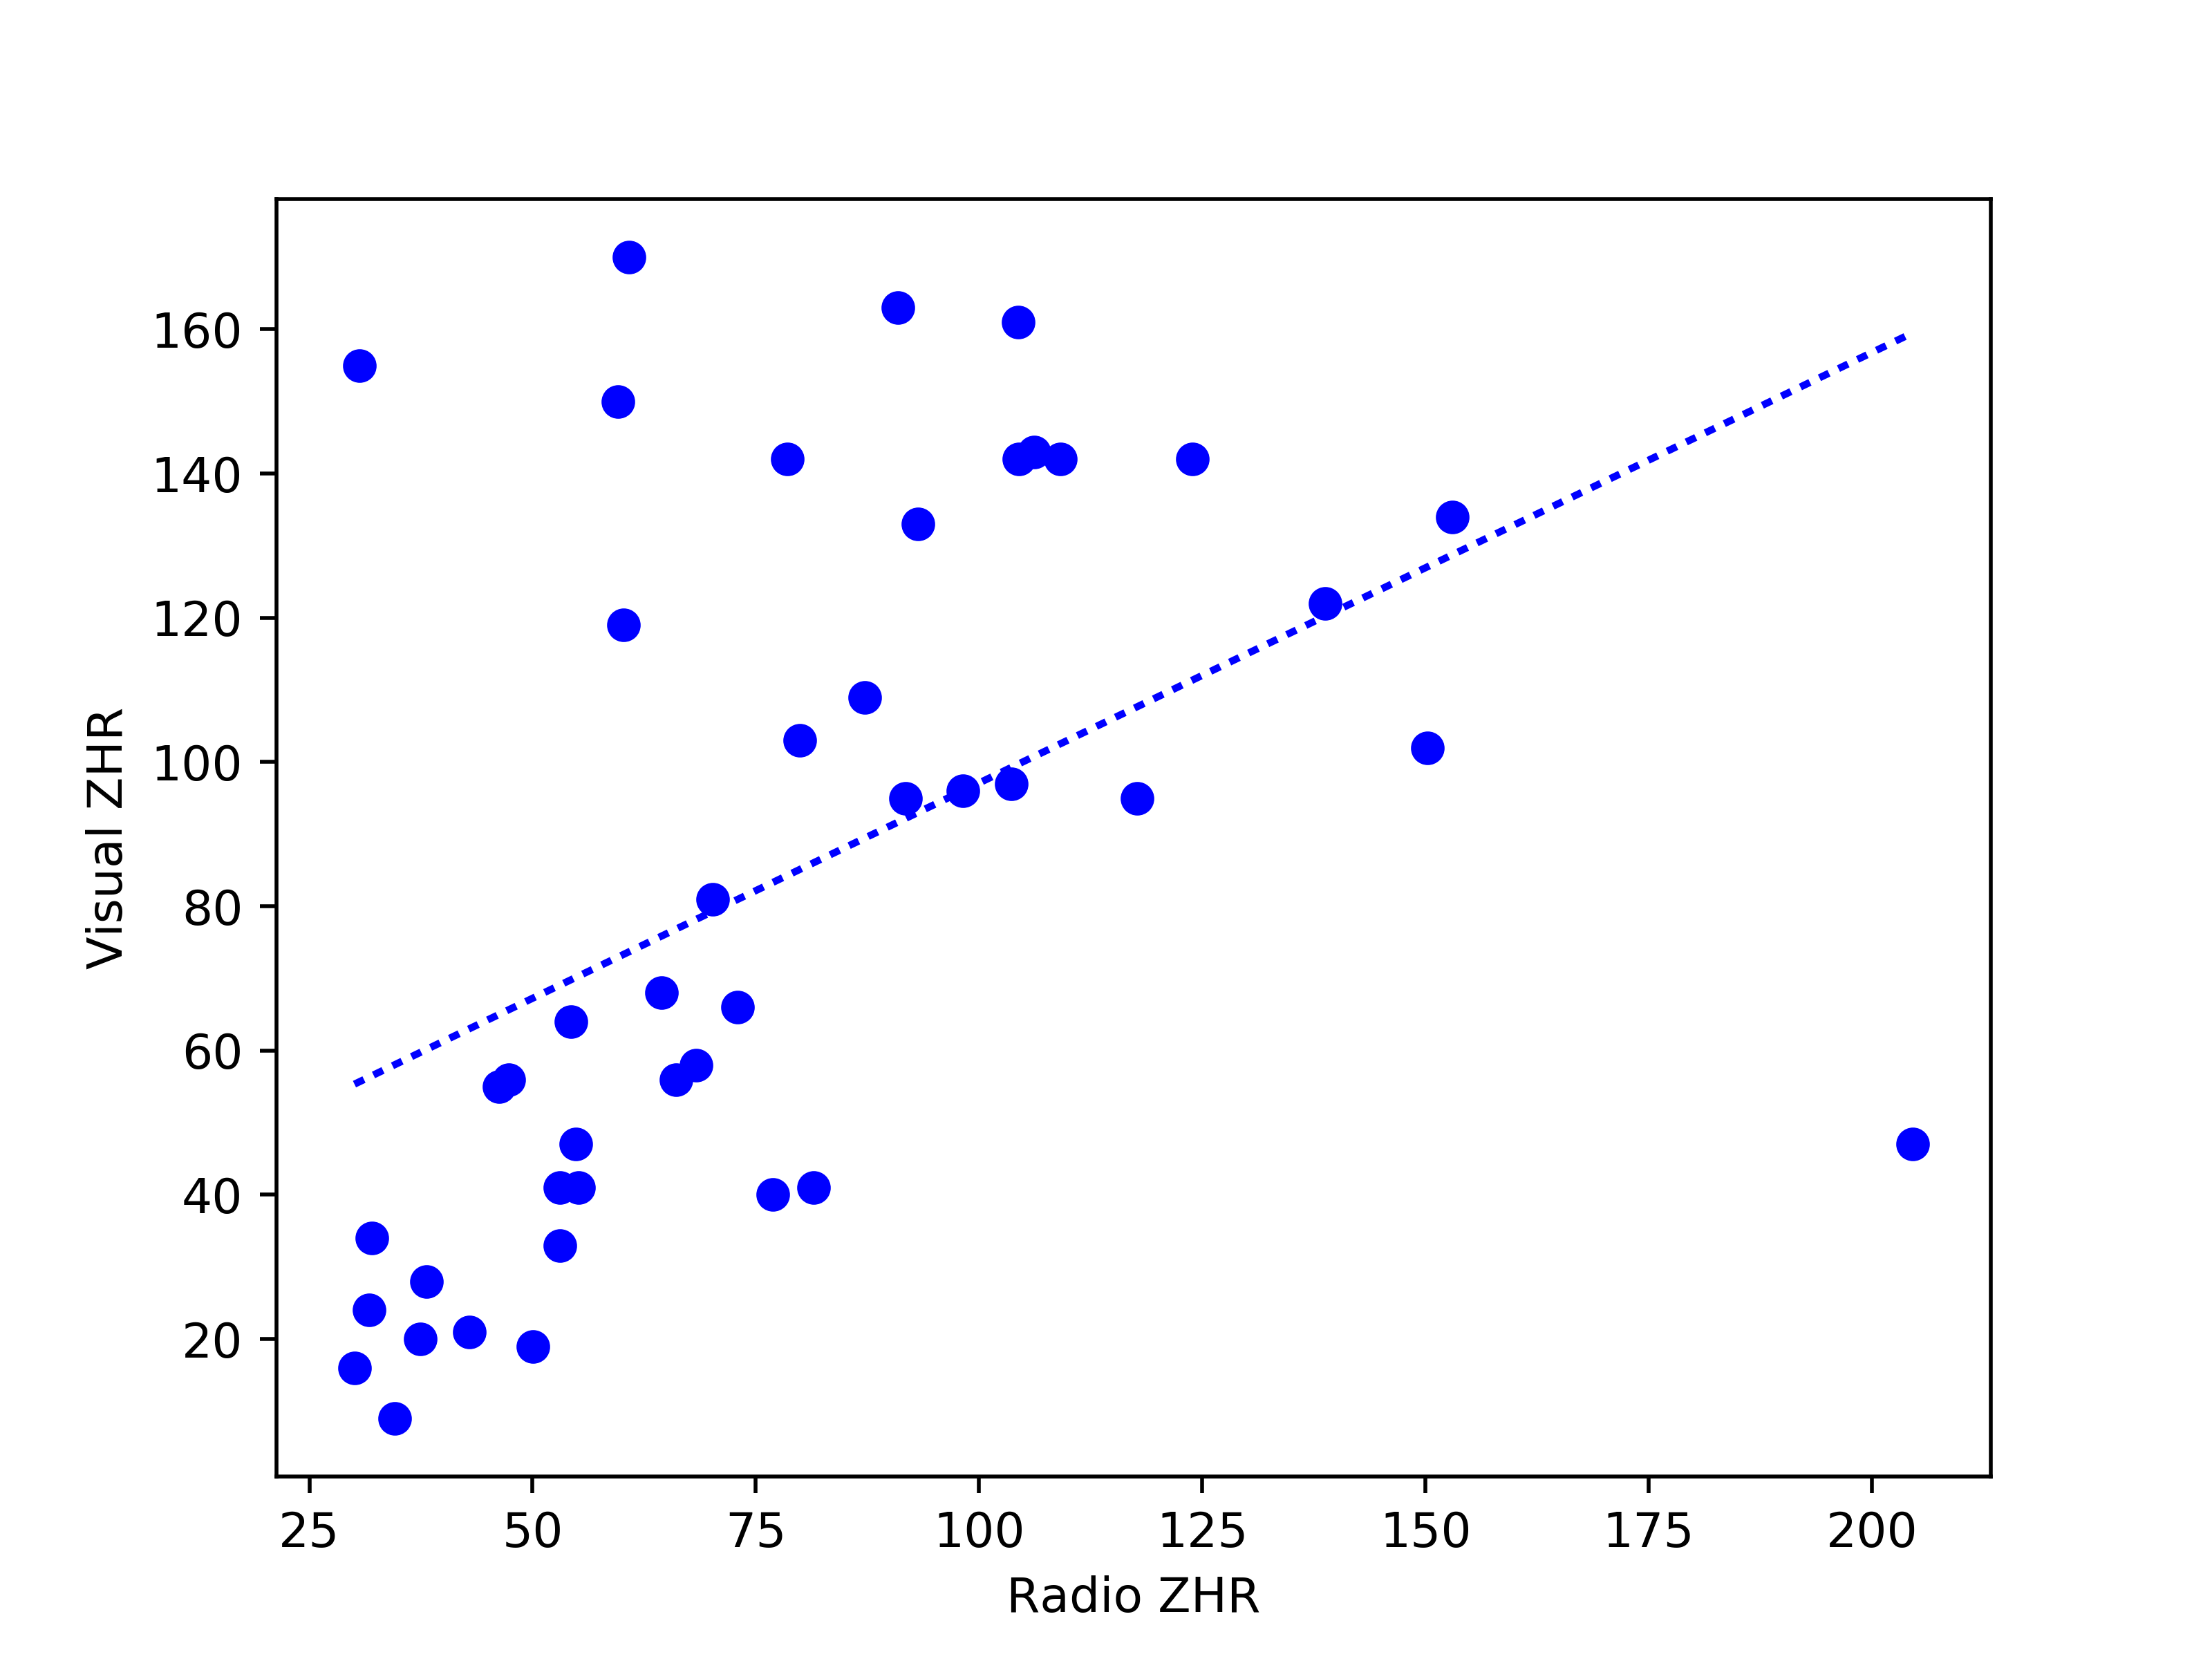
\includegraphics[width=\linewidth]{peak_scatter}
	\end{frame}

	\begin{frame}
		\centering
		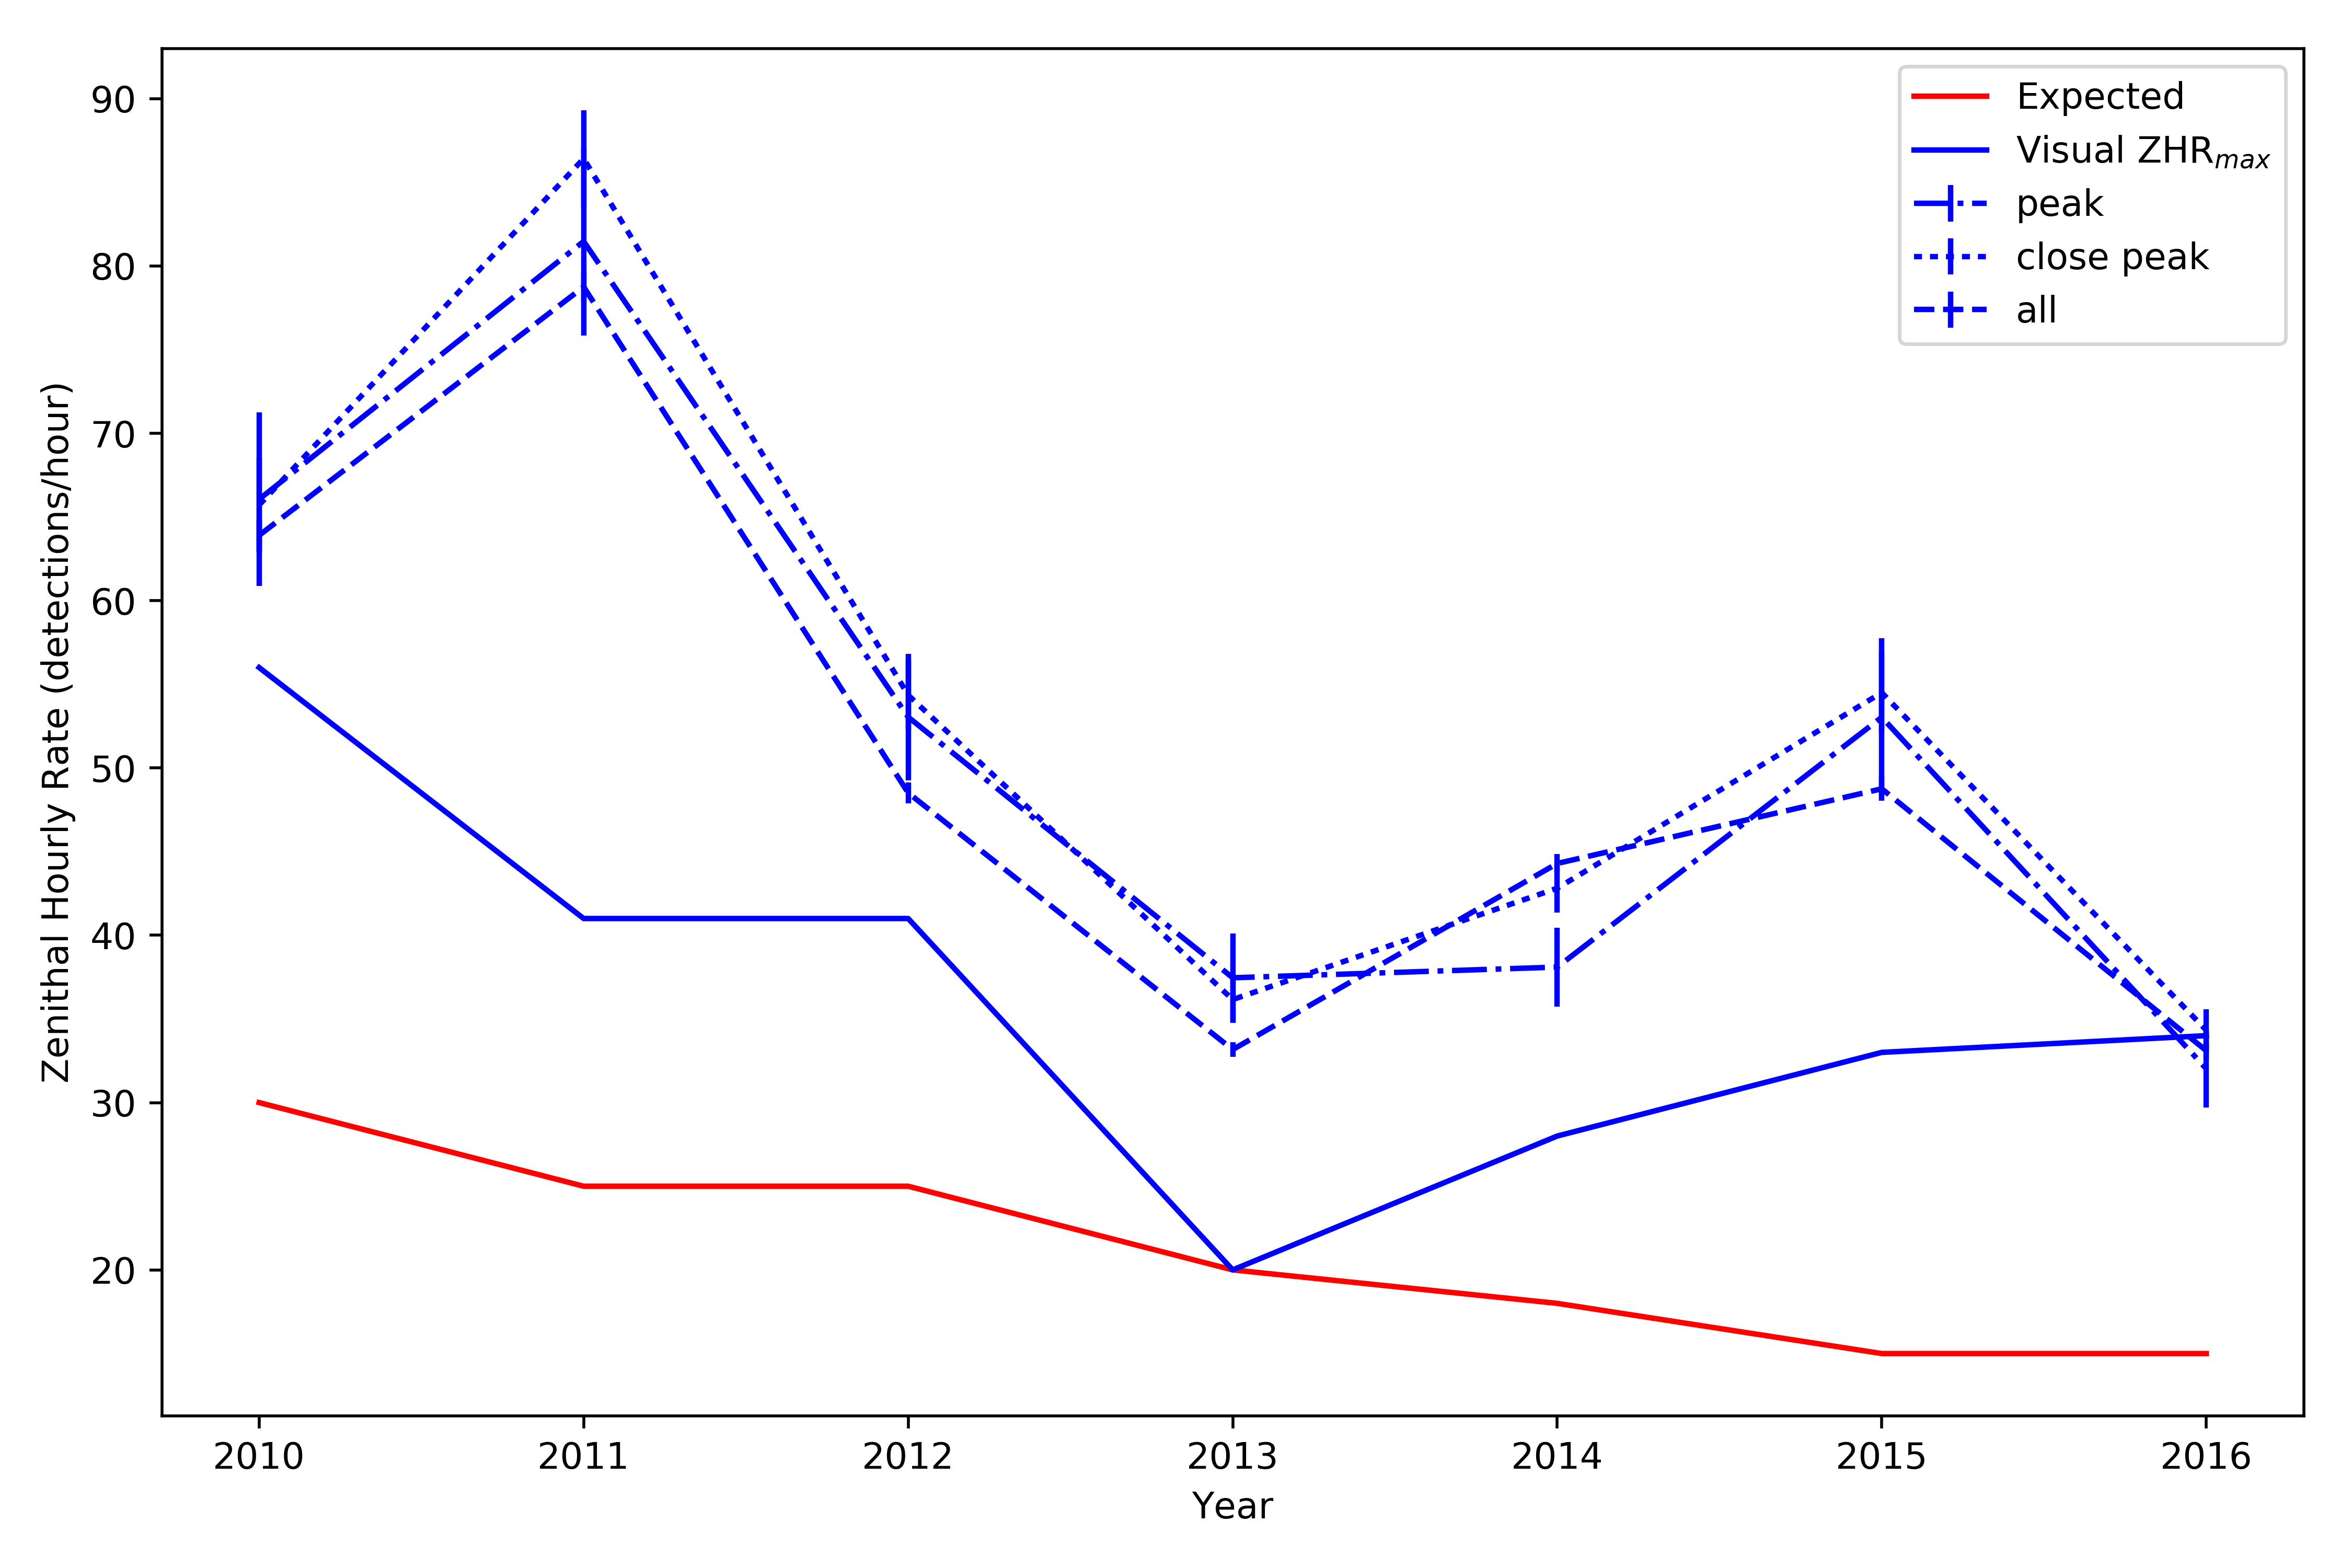
\includegraphics[width=\linewidth]{orionids_notitle}
	\end{frame}
	
	\section{Image analysis}
	\begin{frame}
		\centering
		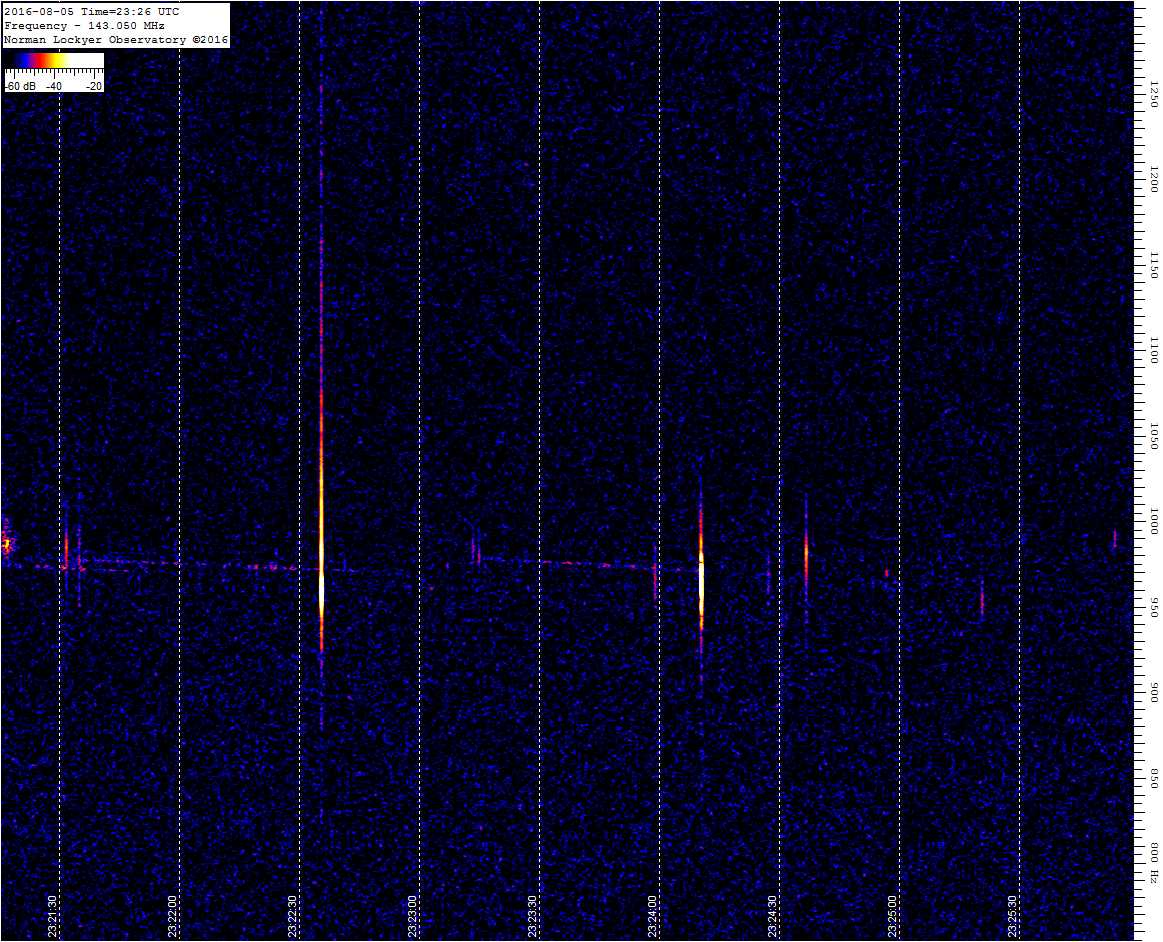
\includegraphics[width=0.9\linewidth]{2D}\\
		\flushleft\credit{Lockyer Technology Centre, NLO}
	\end{frame}

	\begin{frame}
		\centering
		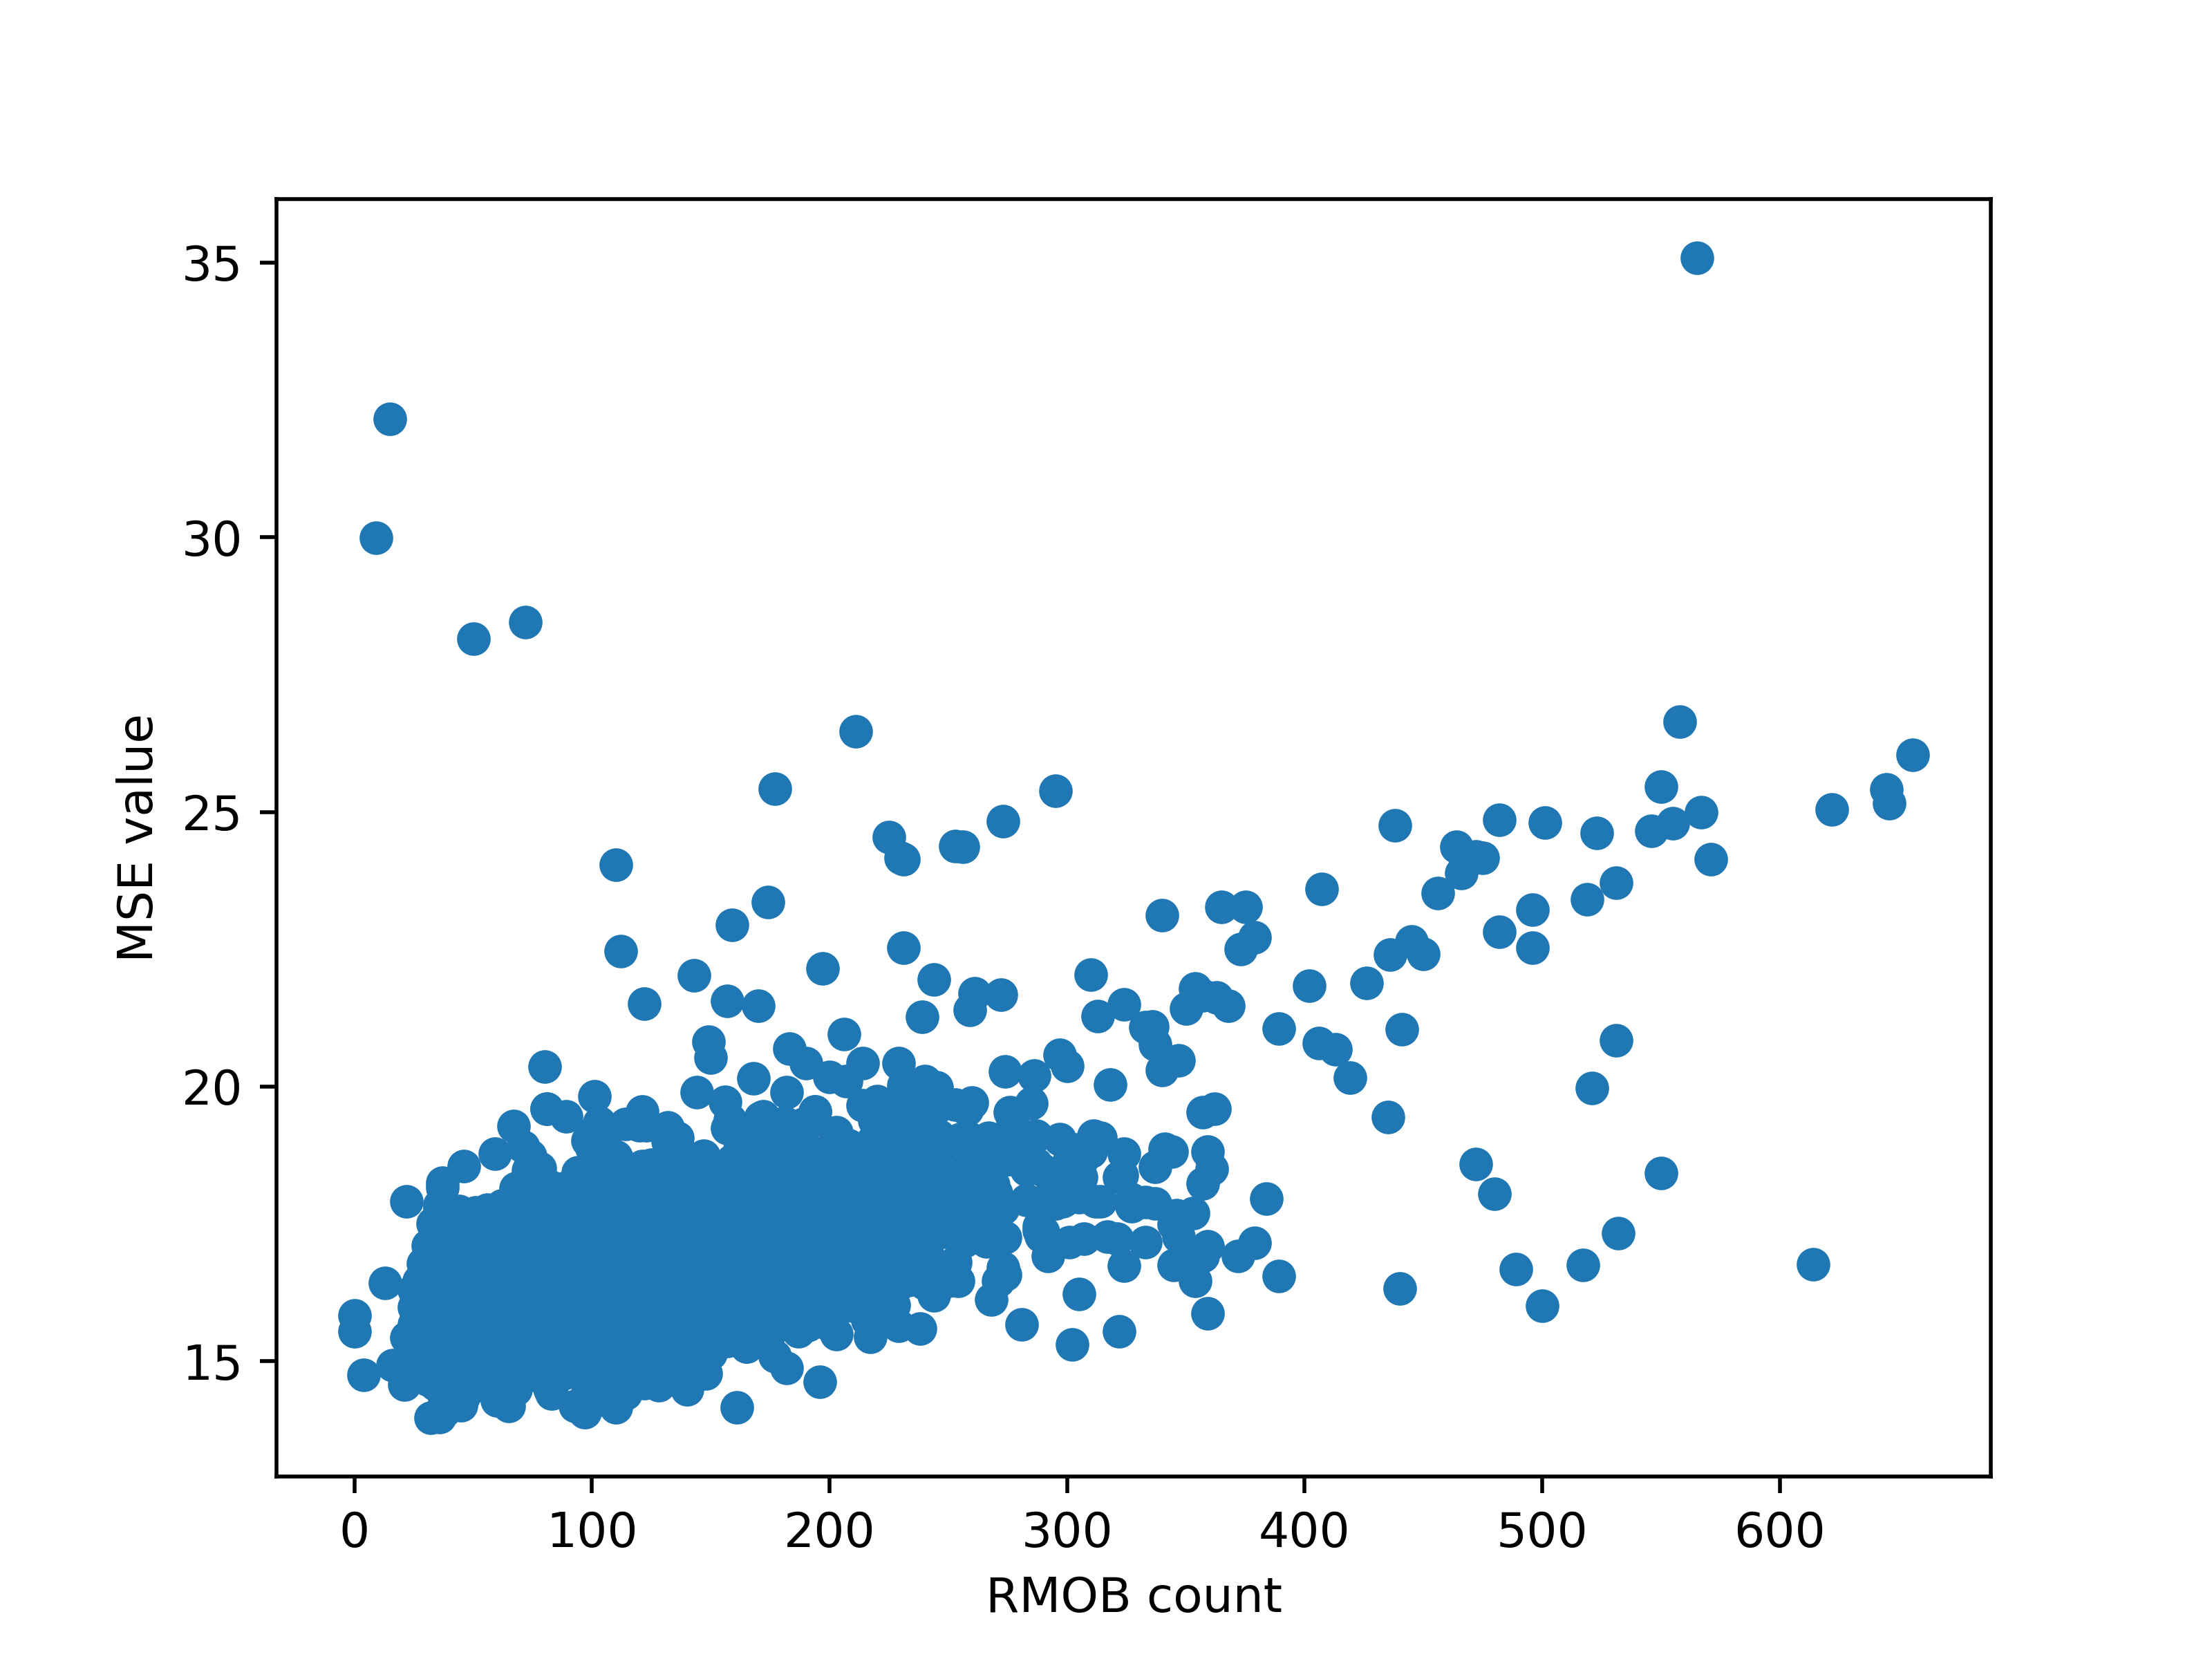
\includegraphics[width=\linewidth]{after}
	\end{frame}

\end{document}
